\setcounter{part}{0}
\setcounter{chapter}{0}
\setcounter{section}{0}
\renewcommand{\thechapter}{\arabic{chapter}}
\renewcommand{\thepart}{\arabic{part}}
\renewcommand{\thesection}{\arabic{section}}
\renewcommand{\thefigure}{A\arabic{figure}}
\renewcommand{\thetable}{A\arabic{table}}
\setcounter{figure}{0}
\setcounter{table}{0}
\appendix
\label{appendix:applications}
\section{Applications développées durant la formation}
\subsection{Application 1 }
\subsubsection{Description}
Cette application est une application qui permet d'afficher les données de météo de la position géographique de l'utilisateur.

\subsubsection{But}
Le but de la developpement de cette application est de metriser la consomation des web services SOAP et integrer des librairies natives de capacitor.


\subsubsection{Fonctionnalités}
\begin{itemize}
    \item Affichage de la météo de la position géographique de l'utilisateur en temps réel.
    \item Affichage de la prévision météo de la position géographique de l'utilisateur.
\end{itemize}

\subsubsection{Réalisations}
La figure suivante montre les captures d'écran de l'application.

\begin{figure}[H]
    \centering
    \fbox{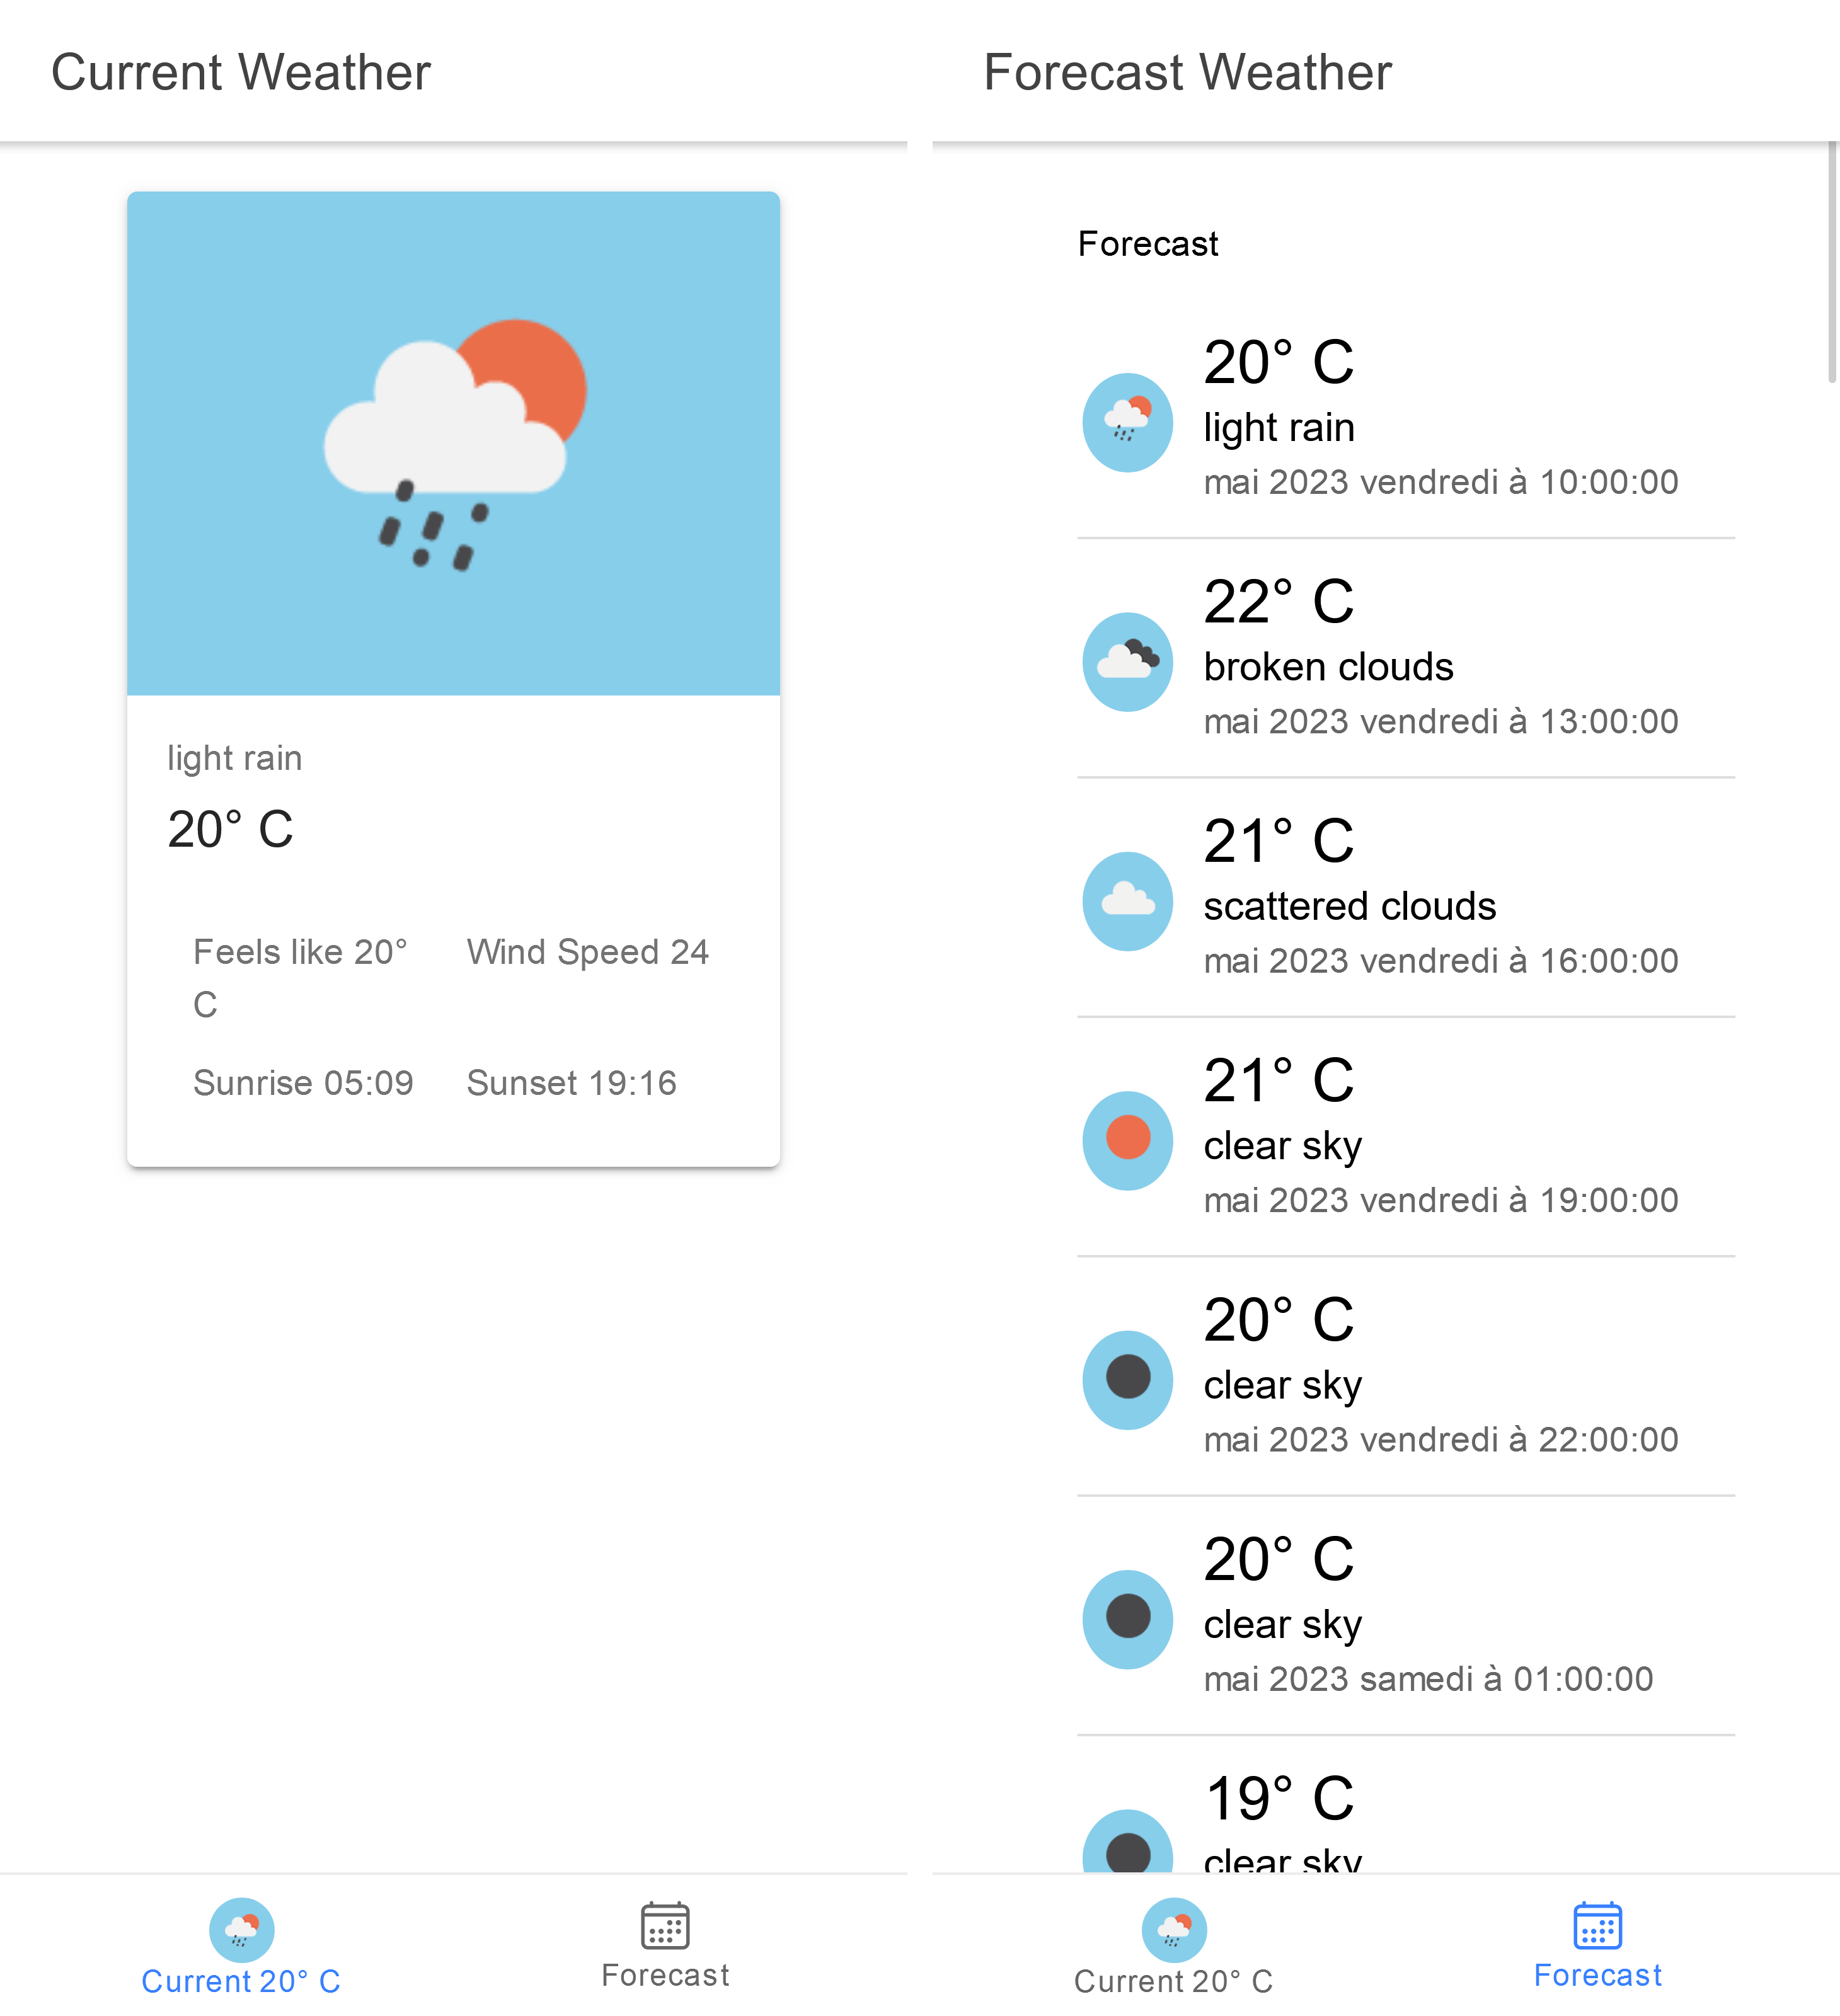
\includegraphics[width=0.4\textwidth]{capture_application_1}}
    \caption{Captures d'écran de l'application 1}
    \label{appendix:capture_app1}
\end{figure}

\subsubsection{Difficultés rencontrées}
\begin{itemize}
    \item La documentation de capacitor est très limitée.
    \item La consommation des web services SOAP a soulevé des erreurs CORS.
\end{itemize}

\subsubsection{Solutions apportées}
\begin{itemize}
    \item Nous avons utilisé les exemples de capacitor pour comprendre son fonctionnement.
    \item Nous avons utilisé un proxy pour contourner les erreurs CORS lors de la développement et HTTPCapacitor pour contourner les erreurs CORS lors de la production.
\end{itemize}

\textbf{HTTPCapacitor} est une librairie qui permet d'envoyer des requêtes HTTP nativement depuis capacitor.

\subsection{Application 2 }

\subsubsection{Description}
Cette application est une application mobile qui permet de créer des images de signature.

\subsubsection{But}
Le but de la developpement de cette application est de découvrir les solutions possibles pour créer des images de signature.

\subsubsection{Fonctionnalités}
\begin{itemize}
    \item Création d'une image de signature.
    \item Affichage de l'image de signature.
    \item Suppression de l'image de signature.
\end{itemize}

\subsubsection{Choix technologiques}
Nous avons testé deux librairies pour créer des images de signature : \textbf{v-perfect-signature} et \textbf{vue-signature-pad}.

% v-perfect-signature vs  vue-signature-pad
\begin{table}[H]
    \caption{Comparaison entre v-perfect-signature et vue-signature-pad}
    \label{tab:v-perfect-signature_vs_vue-signature-pad}
    \centering
    
    \begin{tabular}{|l|l|l|}
    \hline
    \textbf{Librairie} & \textbf{v-perfect-signature} & \textbf{vue-signature-pad} \\ \hline
    \textbf{Documentation} & 
    \begin{tabular}[c]{@{}l@{}}La documentation est \\ très limitée\end{tabular} & 
    \begin{tabular}[c]{@{}l@{}}La documentation est \\ complète\end{tabular} \\ \hline
    \textbf{Maintenance} & 
    \begin{tabular}[c]{@{}l@{}}La librairie n'est pas \\ maintenue\end{tabular} & 
    \begin{tabular}[c]{@{}l@{}}La librairie est \\ maintenue\end{tabular} \\ \hline
    \textbf{Intégration} & 
    \begin{tabular}[c]{@{}l@{}}L'intégration de la \\ librairie est \\ compliquée\end{tabular} & 
    \begin{tabular}[c]{@{}l@{}}L'intégration de la \\ librairie est \\ facile\end{tabular} \\ \hline
    \end{tabular}
    
\end{table}

Nous avons choisi la librairie \textbf{vue-signature-pad} pour créer des images de signature car elle est bien documentée et maintenue.


\subsubsection{Réalisations}
La figure suivante montre les captures d'écran de l'application.

\begin{figure}[H]
    \centering
    \fbox{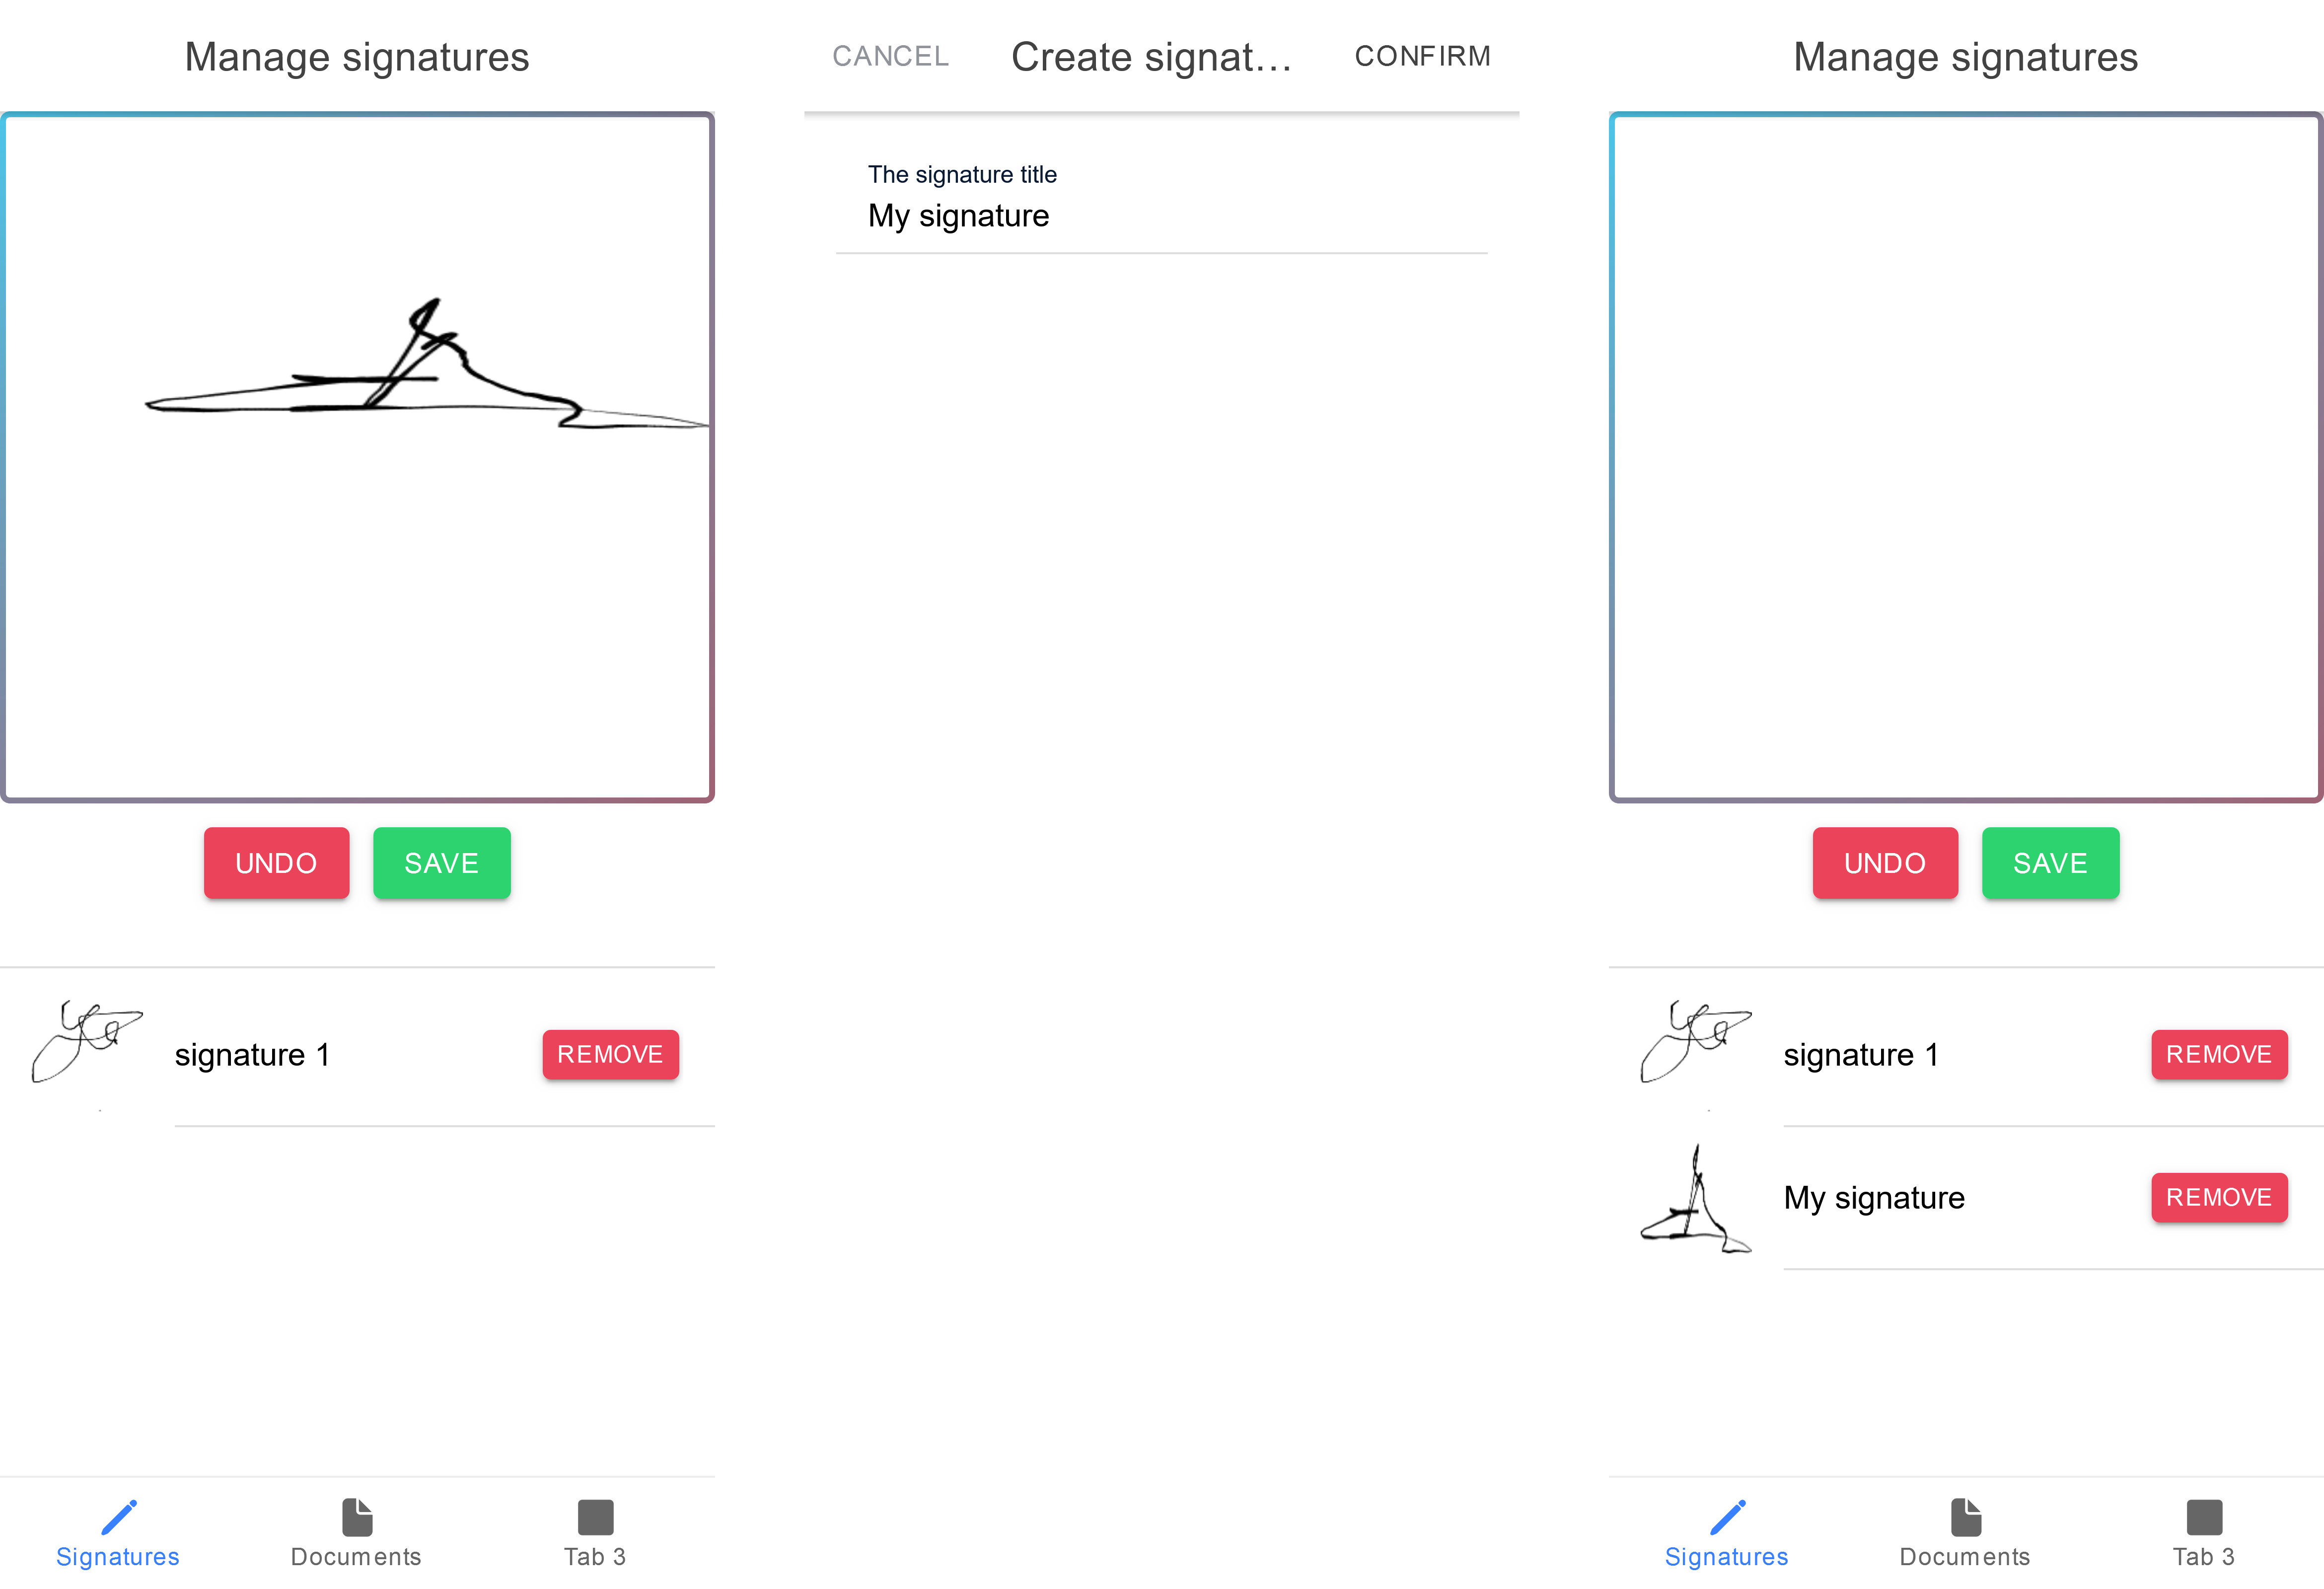
\includegraphics[width=0.6\textwidth]{capture_application_2}}
    \caption{Captures d'écran de l'application 2}
    \label{appendix:capture_app2}
\end{figure}

\subsection{Application 3 }

\subsubsection{Description}
Cette application est une application mobile qui permet d'afficher un fichier PDF.

\subsubsection{But}
Le but de la developpement de cette application est de découvrir les solutions possibles pour afficher des fichiers PDF.

\subsubsection{Fonctionnalités}
\begin{itemize}
    \item Affichage d'un fichier PDF.
    \item Navigation entre les pages du fichier PDF.
\end{itemize}

\subsubsection{Choix technologiques}

% vue-pdf vs pdfvuer 
Pour afficher des fichiers PDF, nous avons testé deux librairies : \textbf{vue-pdf} et \textbf{pdfvuer}.
\begin{table}[H]
    \caption{Comparaison entre vue-pdf et pdfvuer}
    \label{tab:vpdf_pdfvuer}
    \centering
    
    \begin{tabular}{|l|l|l|}
    \hline
    \textbf{Librairie} & \textbf{pdfvuer} & \textbf{vue-pdf} \\ \hline
    \textbf{Documentation} & 
    \begin{tabular}[c]{@{}l@{}}Manque de documentation \end{tabular} & 
    \begin{tabular}[c]{@{}l@{}}La documentation est \\ complète\end{tabular} \\ \hline
    \textbf{Maintenance} & 
    \begin{tabular}[c]{@{}l@{}}La librairie n'est pas \\ maintenue\end{tabular} & 
    \begin{tabular}[c]{@{}l@{}}La librairie est \\ maintenue\end{tabular} \\ \hline
    \textbf{Intégration} & 
    \begin{tabular}[c]{@{}l@{}}L'intégration de la \\ librairie est \\ facile\end{tabular} & 
    \begin{tabular}[c]{@{}l@{}}L'intégration de la \\ librairie est \\ facile\end{tabular} \\ \hline
    \end{tabular}
    
\end{table}

Nous avons choisi la librairie \textbf{vue-pdf} pour afficher des fichiers PDF car elle est bien documentée et maintenue.

\subsubsection{Réalisations}

La figure suivante montre une capture d'écran de l'application.

\begin{figure}[H]
    \centering
    \fbox{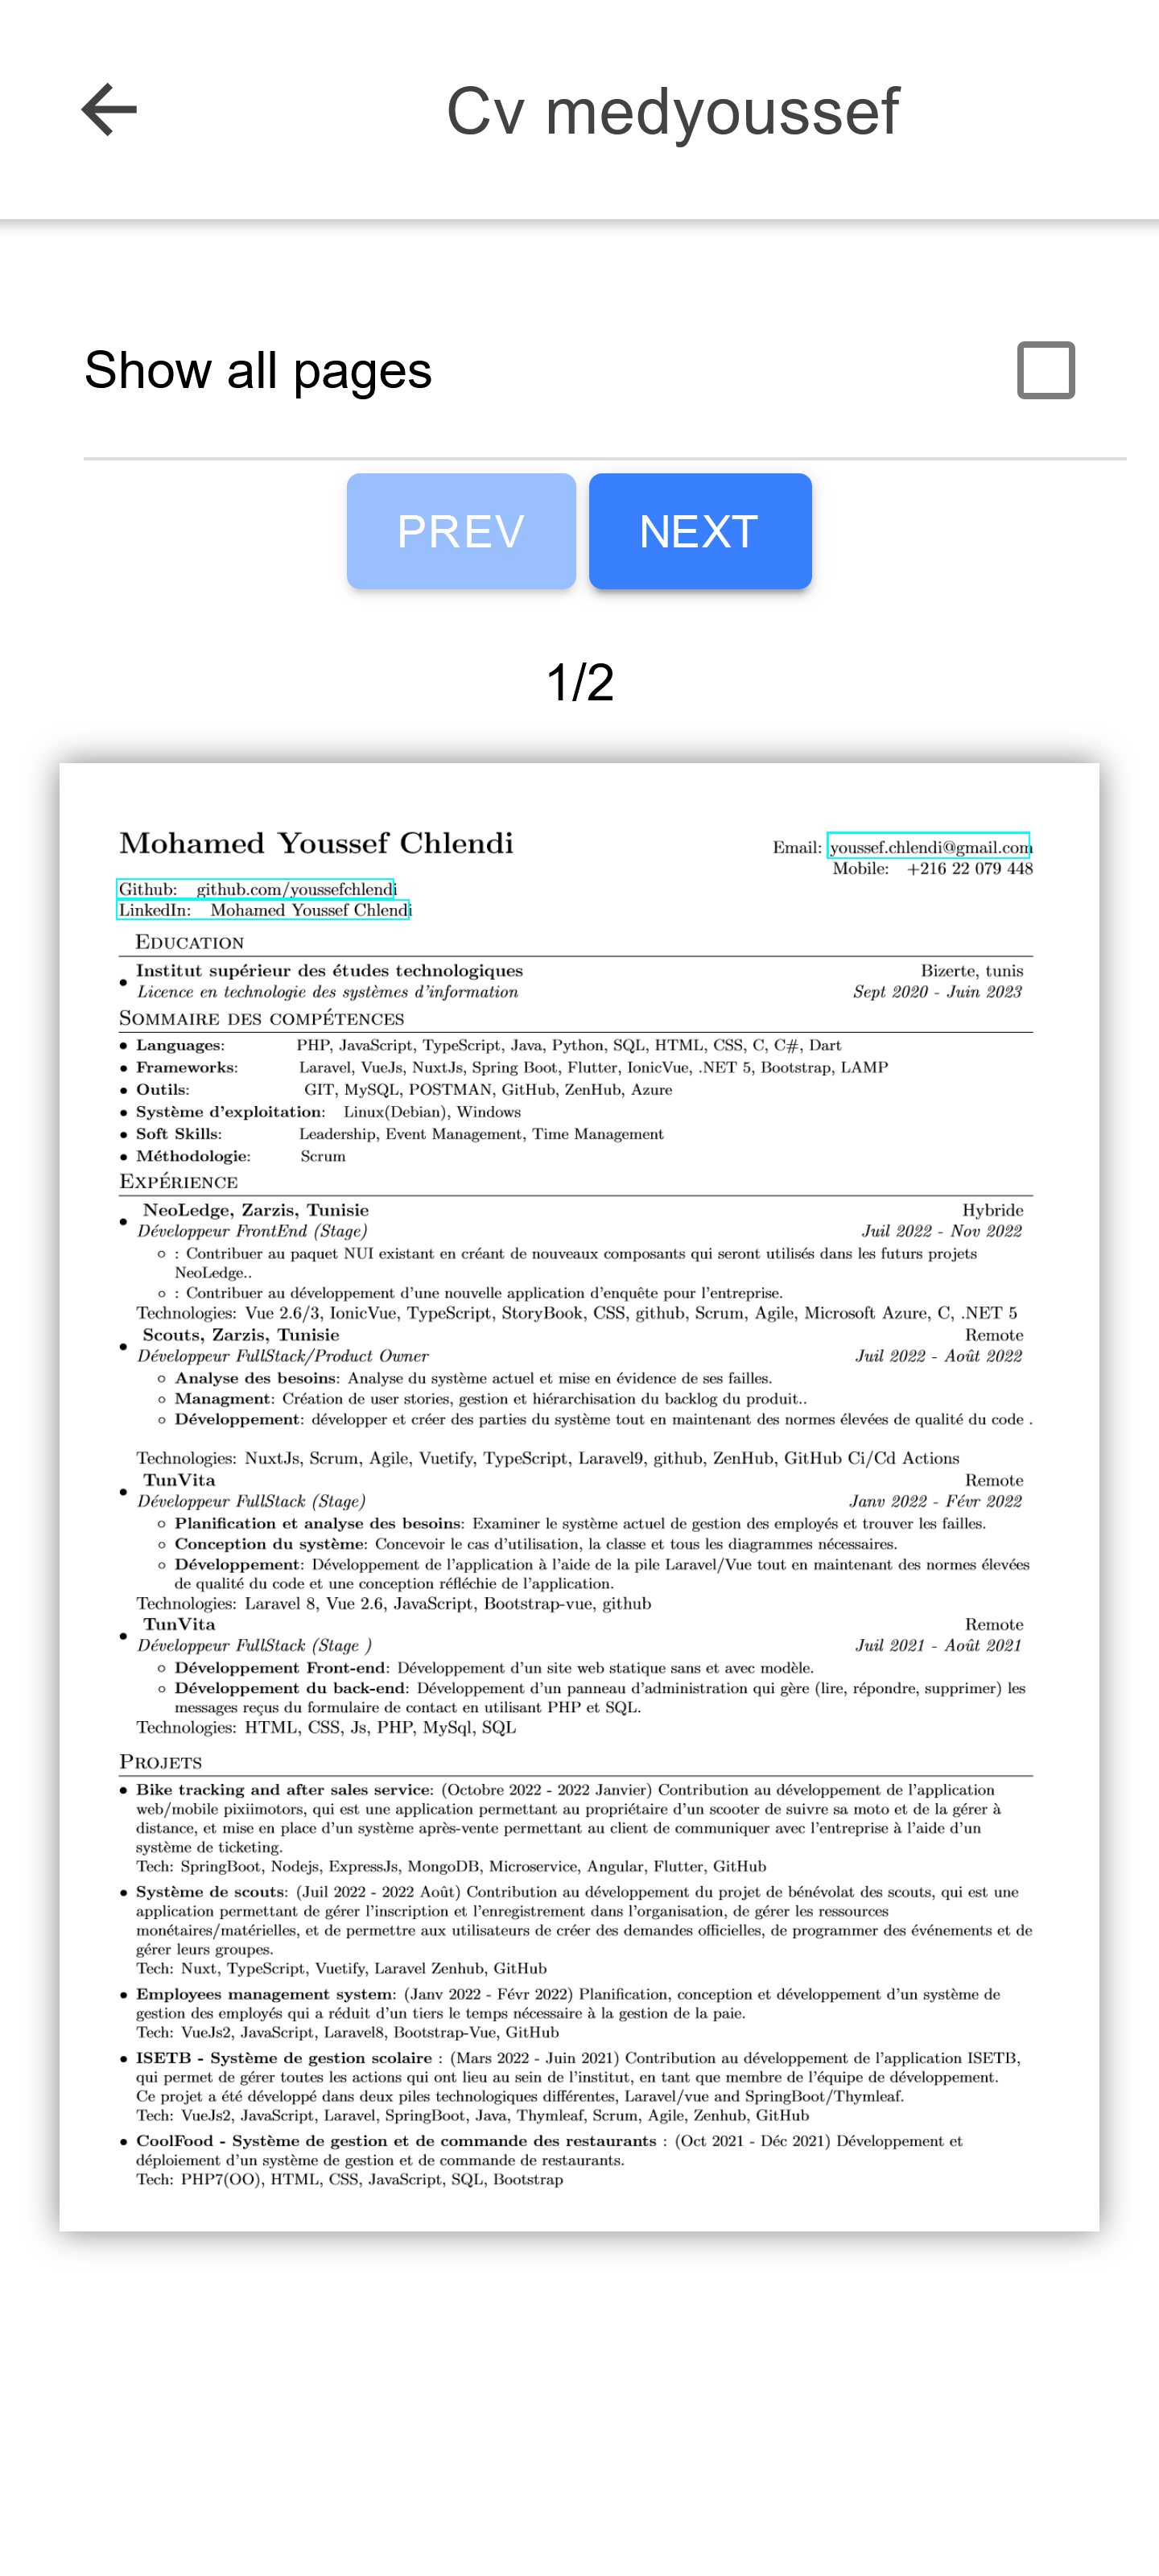
\includegraphics[width=0.2\textwidth]{capture_application_3}}
    \caption{Capture d'écran de l'application 3}
    \label{appendix:capture_app3}
\end{figure}

\subsection{Application 4 }

\subsubsection{Description}
% application importe pdf, gestion signature et signer pdf
Cette application est une application mobile qui permet d'importer un fichier PDF, de signer le fichier PDF et de gérer les signatures.

\subsubsection{But}
Le but de la developpement de cette application est de métriser la positionnement des signatures sur un fichier PDF.

\subsubsection{Fonctionnalités}
\begin{itemize}
    \item Importation d'un fichier PDF.
    \item Affichage d'un fichier PDF.
    \item Déplacement sur le fichier PDF.
    \item Ajout d'une signature sur le fichier PDF.
    \item Ajouter une signature à main levée sur le fichier PDF.
    \item Modification de la position d'une signature sur le fichier PDF.
    \item Gestion des signatures.
\end{itemize}

\subsubsection{Réalisations}

La figure suivante montre les captures d'écran de l'application.

\begin{figure}[H]
    \centering
    \fbox{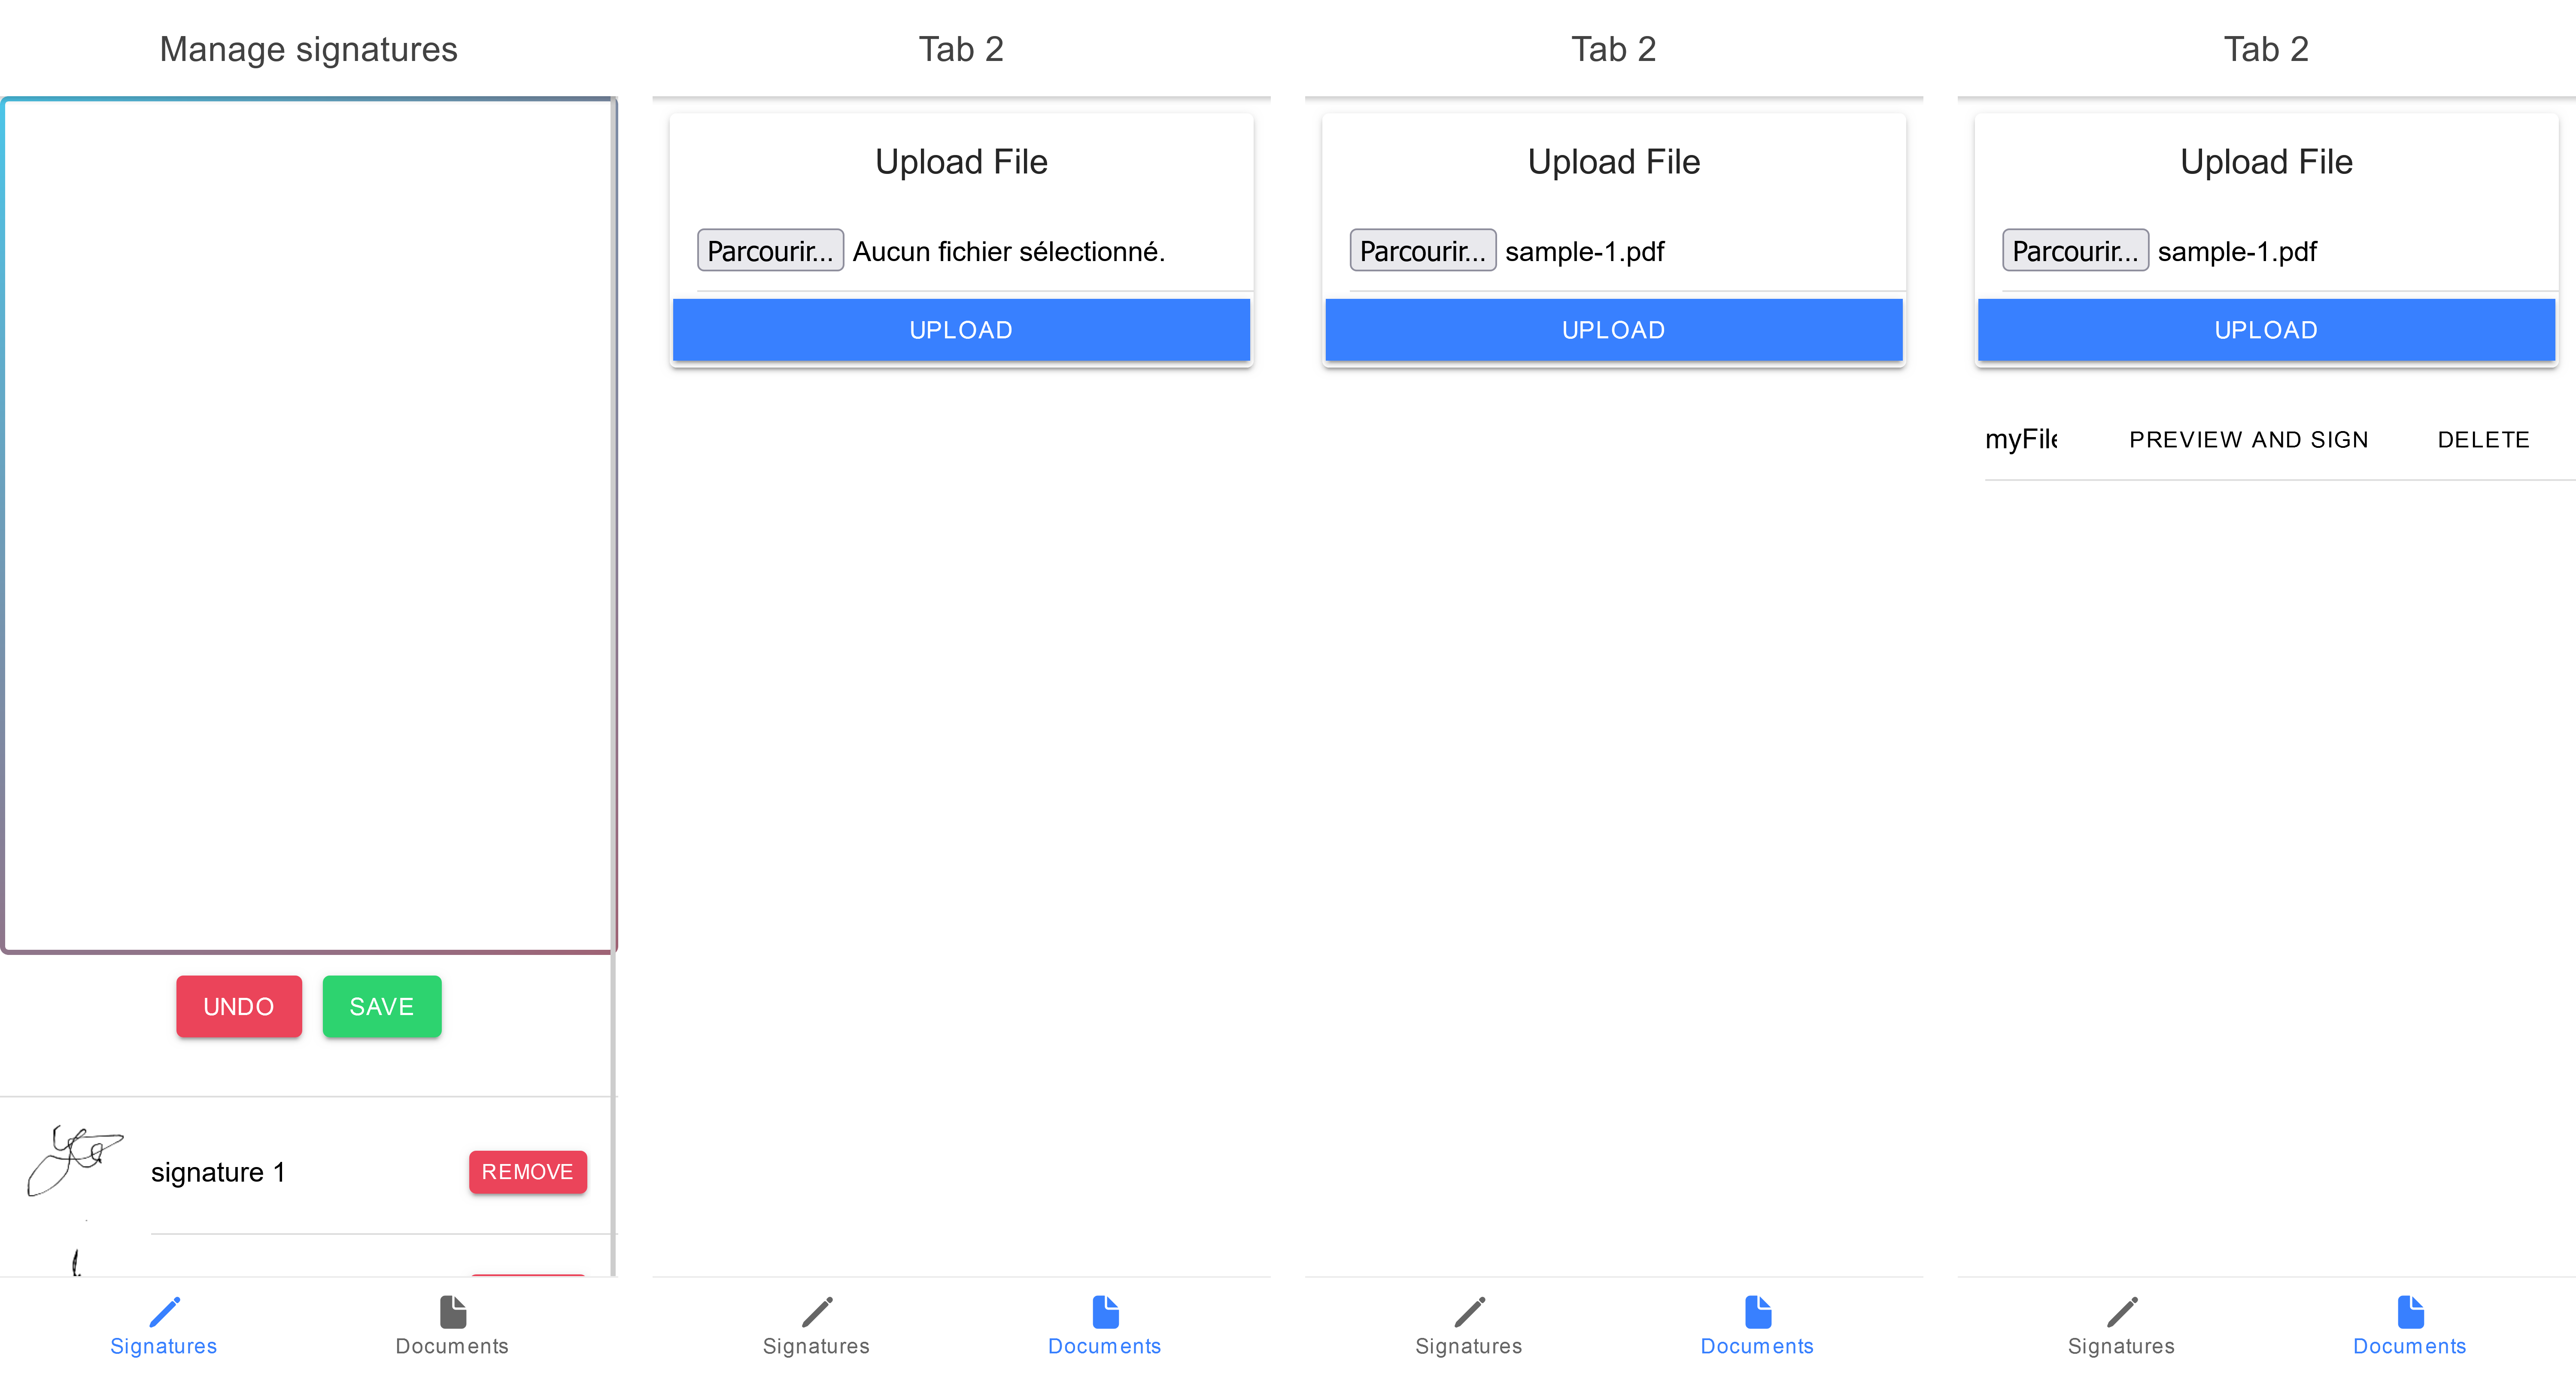
\includegraphics[width=0.6\textwidth]{capture_application_4_1}}
    \caption{Captures de gestion des signatures et documents}
    \label{appendix:capture_app4}
\end{figure}

\begin{figure}[H]
    \centering
    \fbox{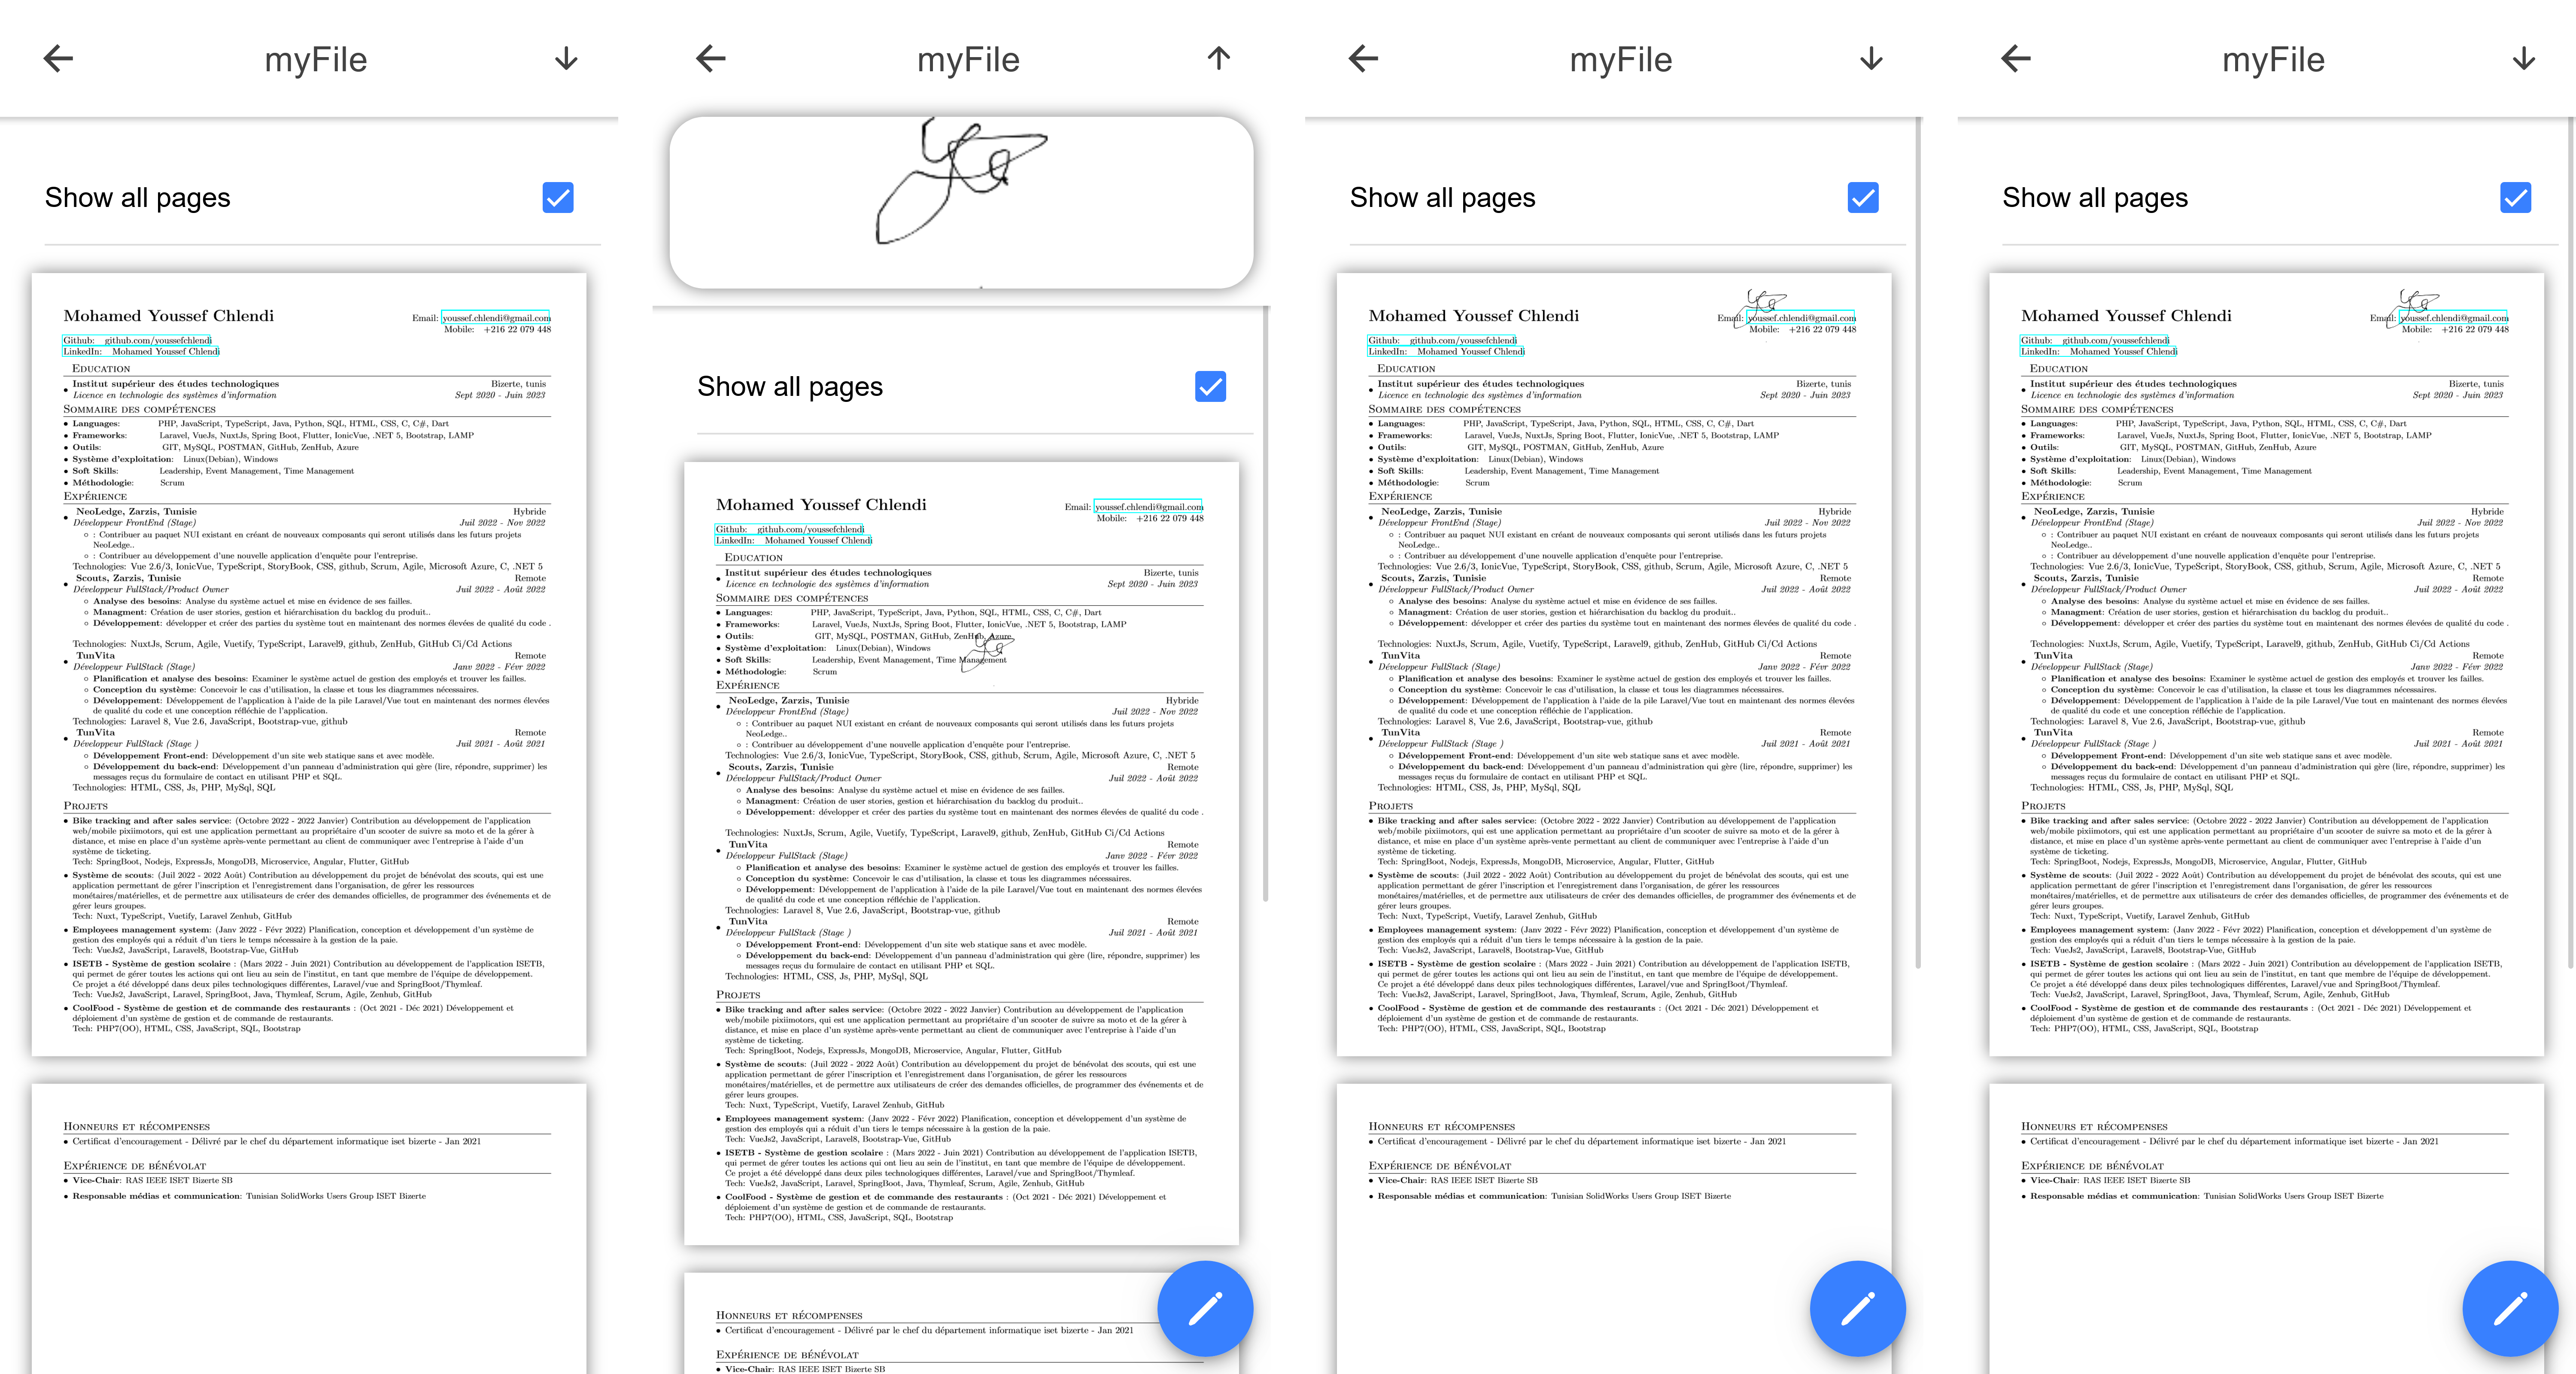
\includegraphics[width=0.6\textwidth]{capture_application_4_2}}
    \caption{Captures de l'affichage et signature d'un document a l'aide d'une image}
    \label{appendix:capture_app4_2}
\end{figure}

\begin{figure}[H]
    \centering
    \fbox{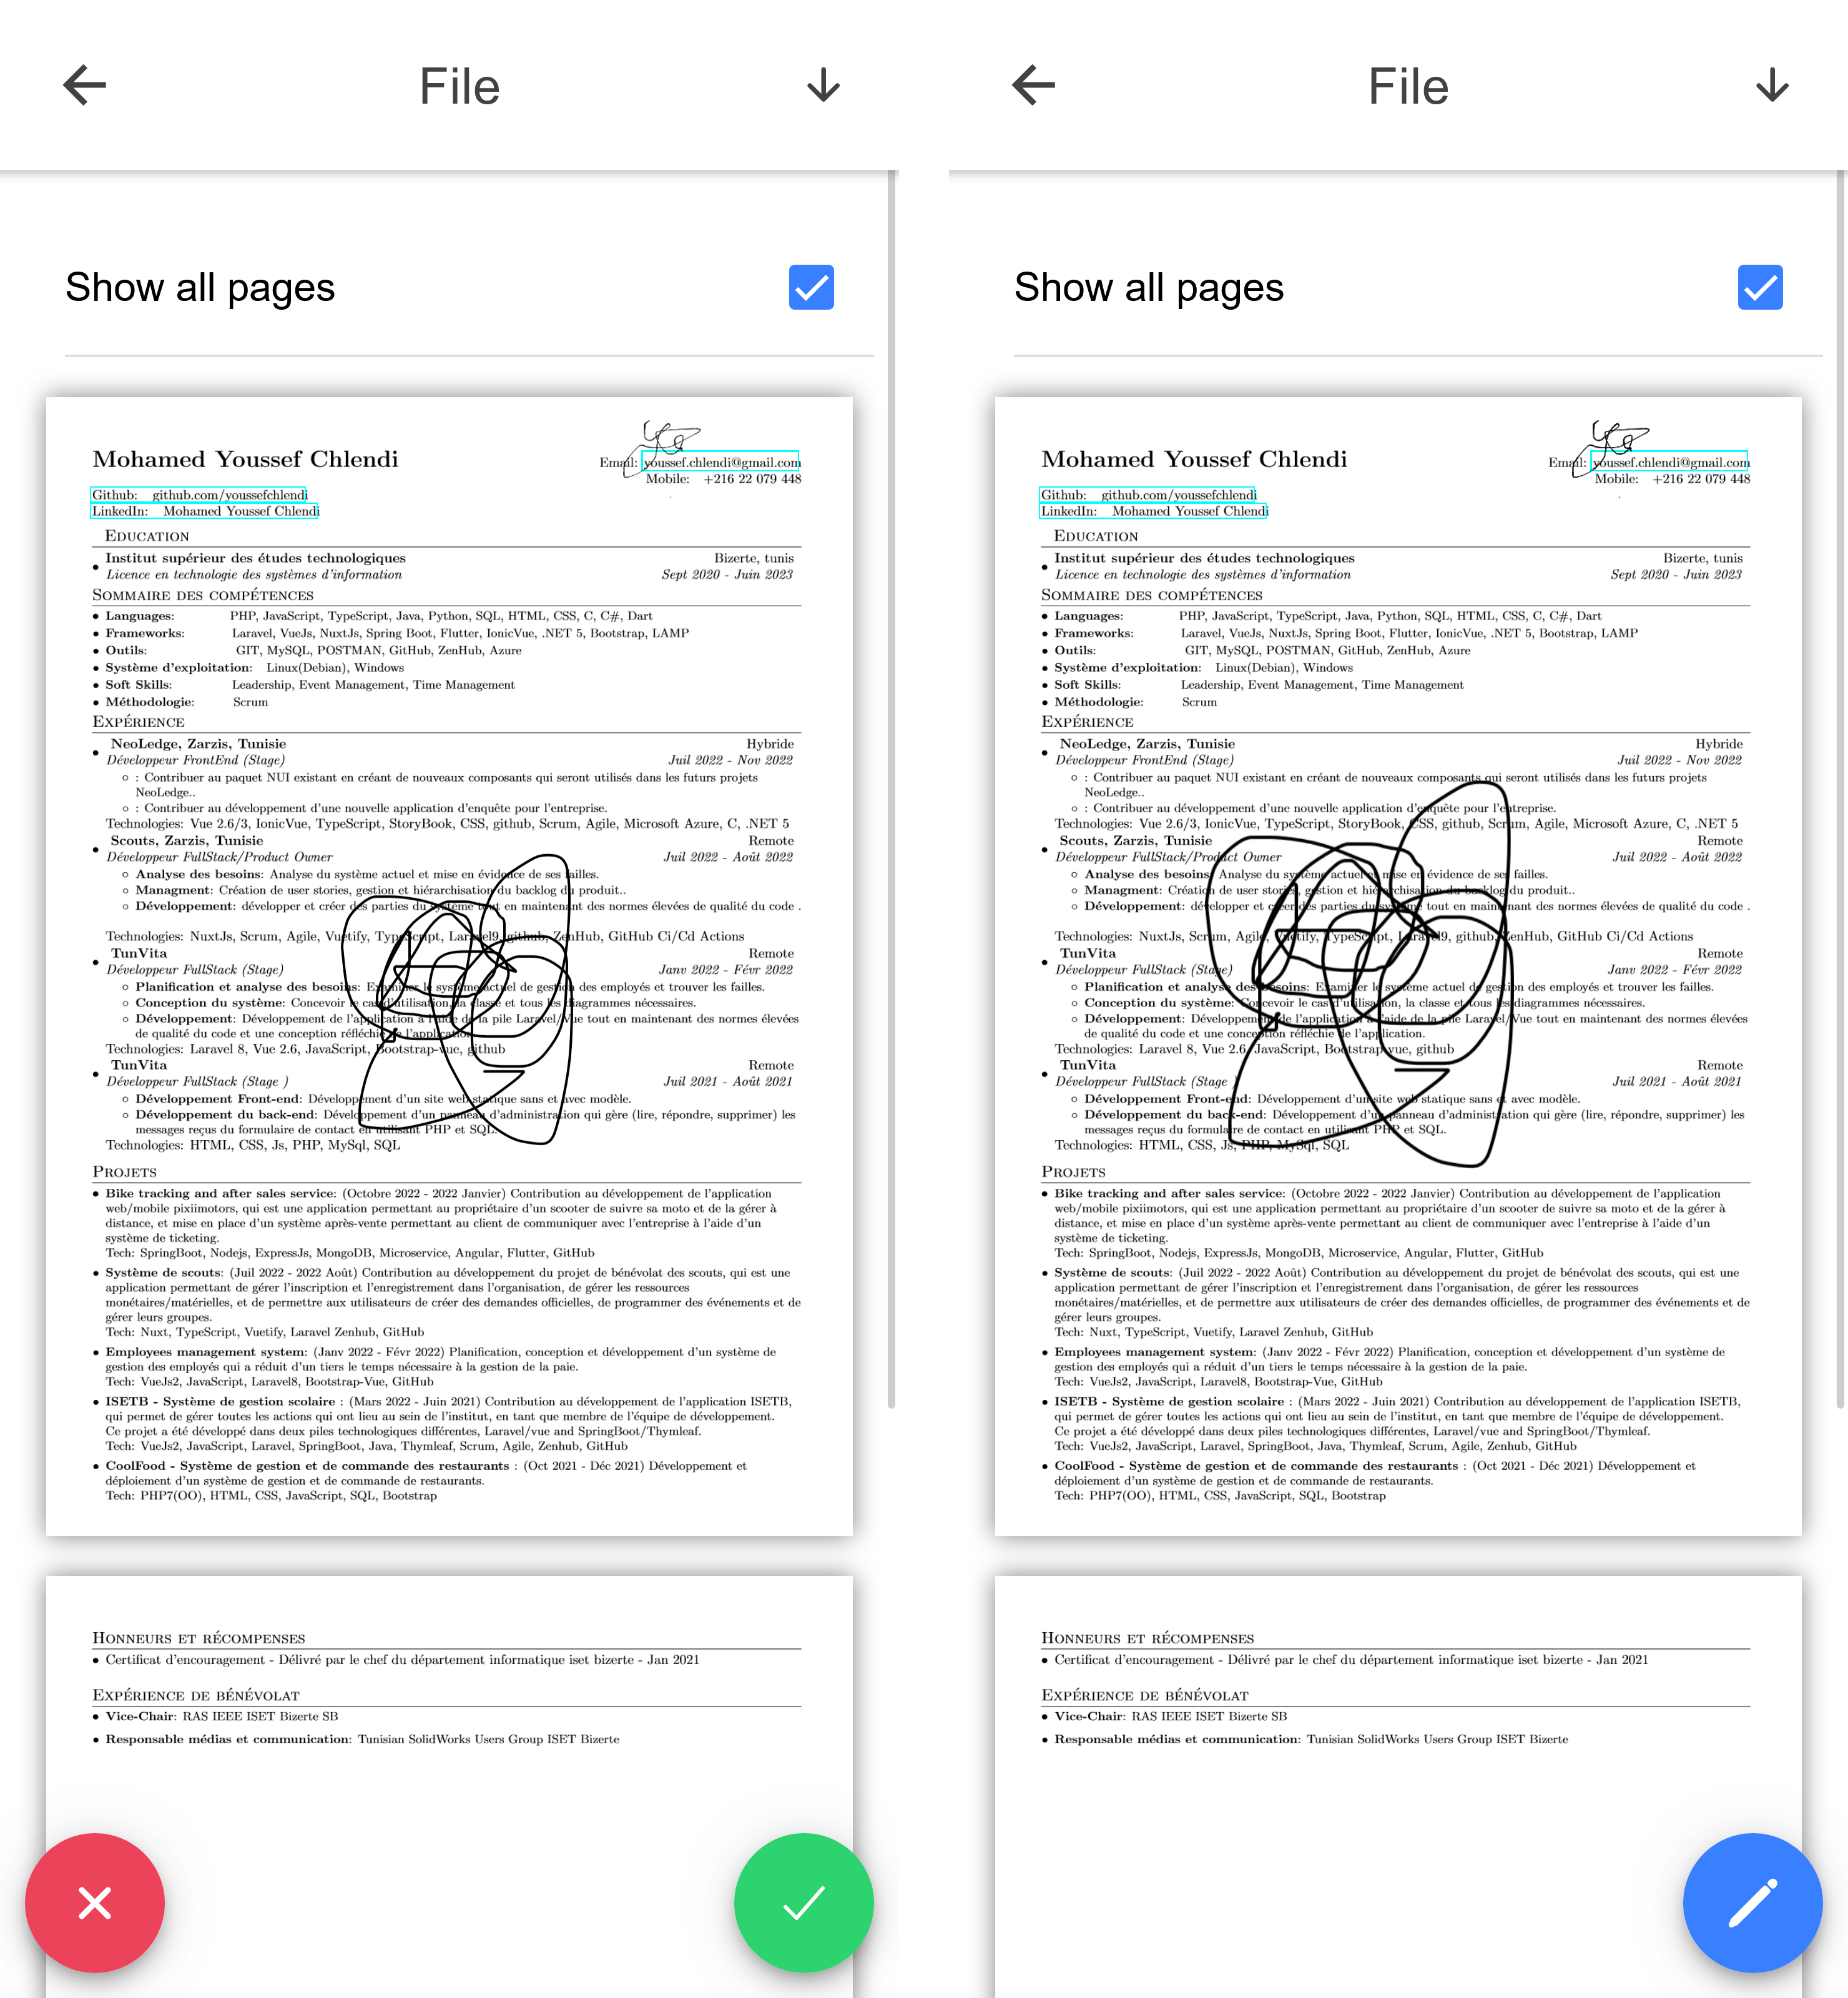
\includegraphics[width=0.4\textwidth]{capture_application_4_3}}
    \caption{Captures de l'affichage et signature d'un document a l'aide d'une signature à main levée}
    \label{appendix:capture_app4_3}
\end{figure}




\section{Capture d'écran de l'application version IOS}

\subsection{Visualisation et signature d’un fichier}
\label{appendix:ios_view_sign}
\begin{figure}[H]
    \centering
    \fbox{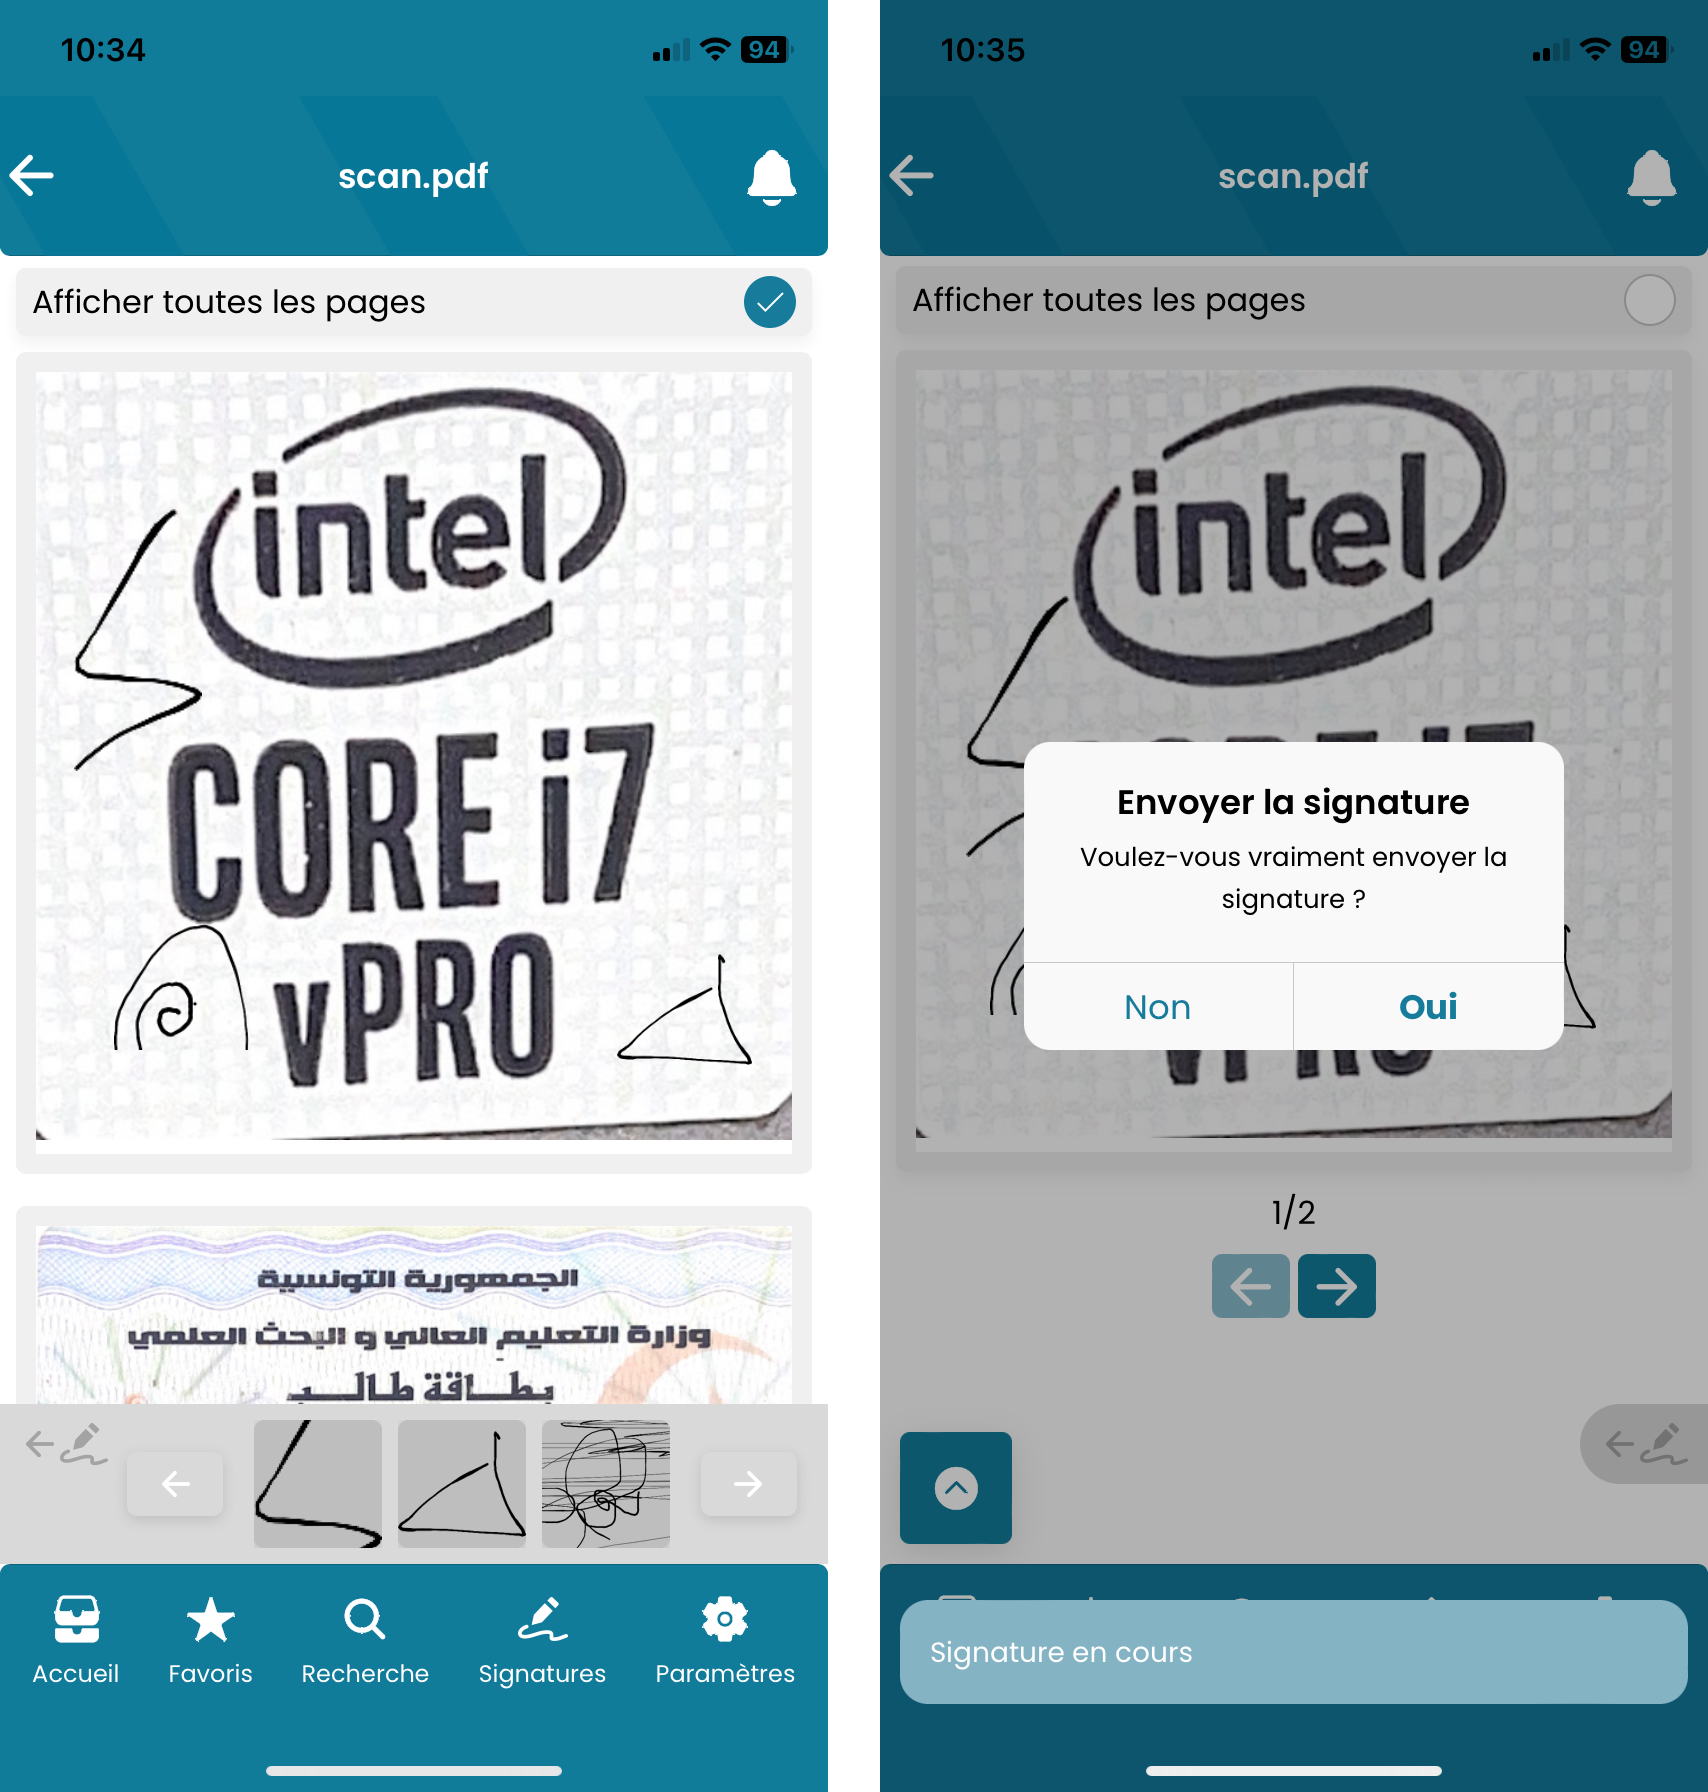
\includegraphics[width=0.4\textwidth]{sign_doc_ios}}
    \caption{Quelques captures d'écran de la signature d’un fichier version IOS}
    \label{appendix:sign_doc_ios}
\end{figure}

\begin{figure}[H]
    \centering
    \fbox{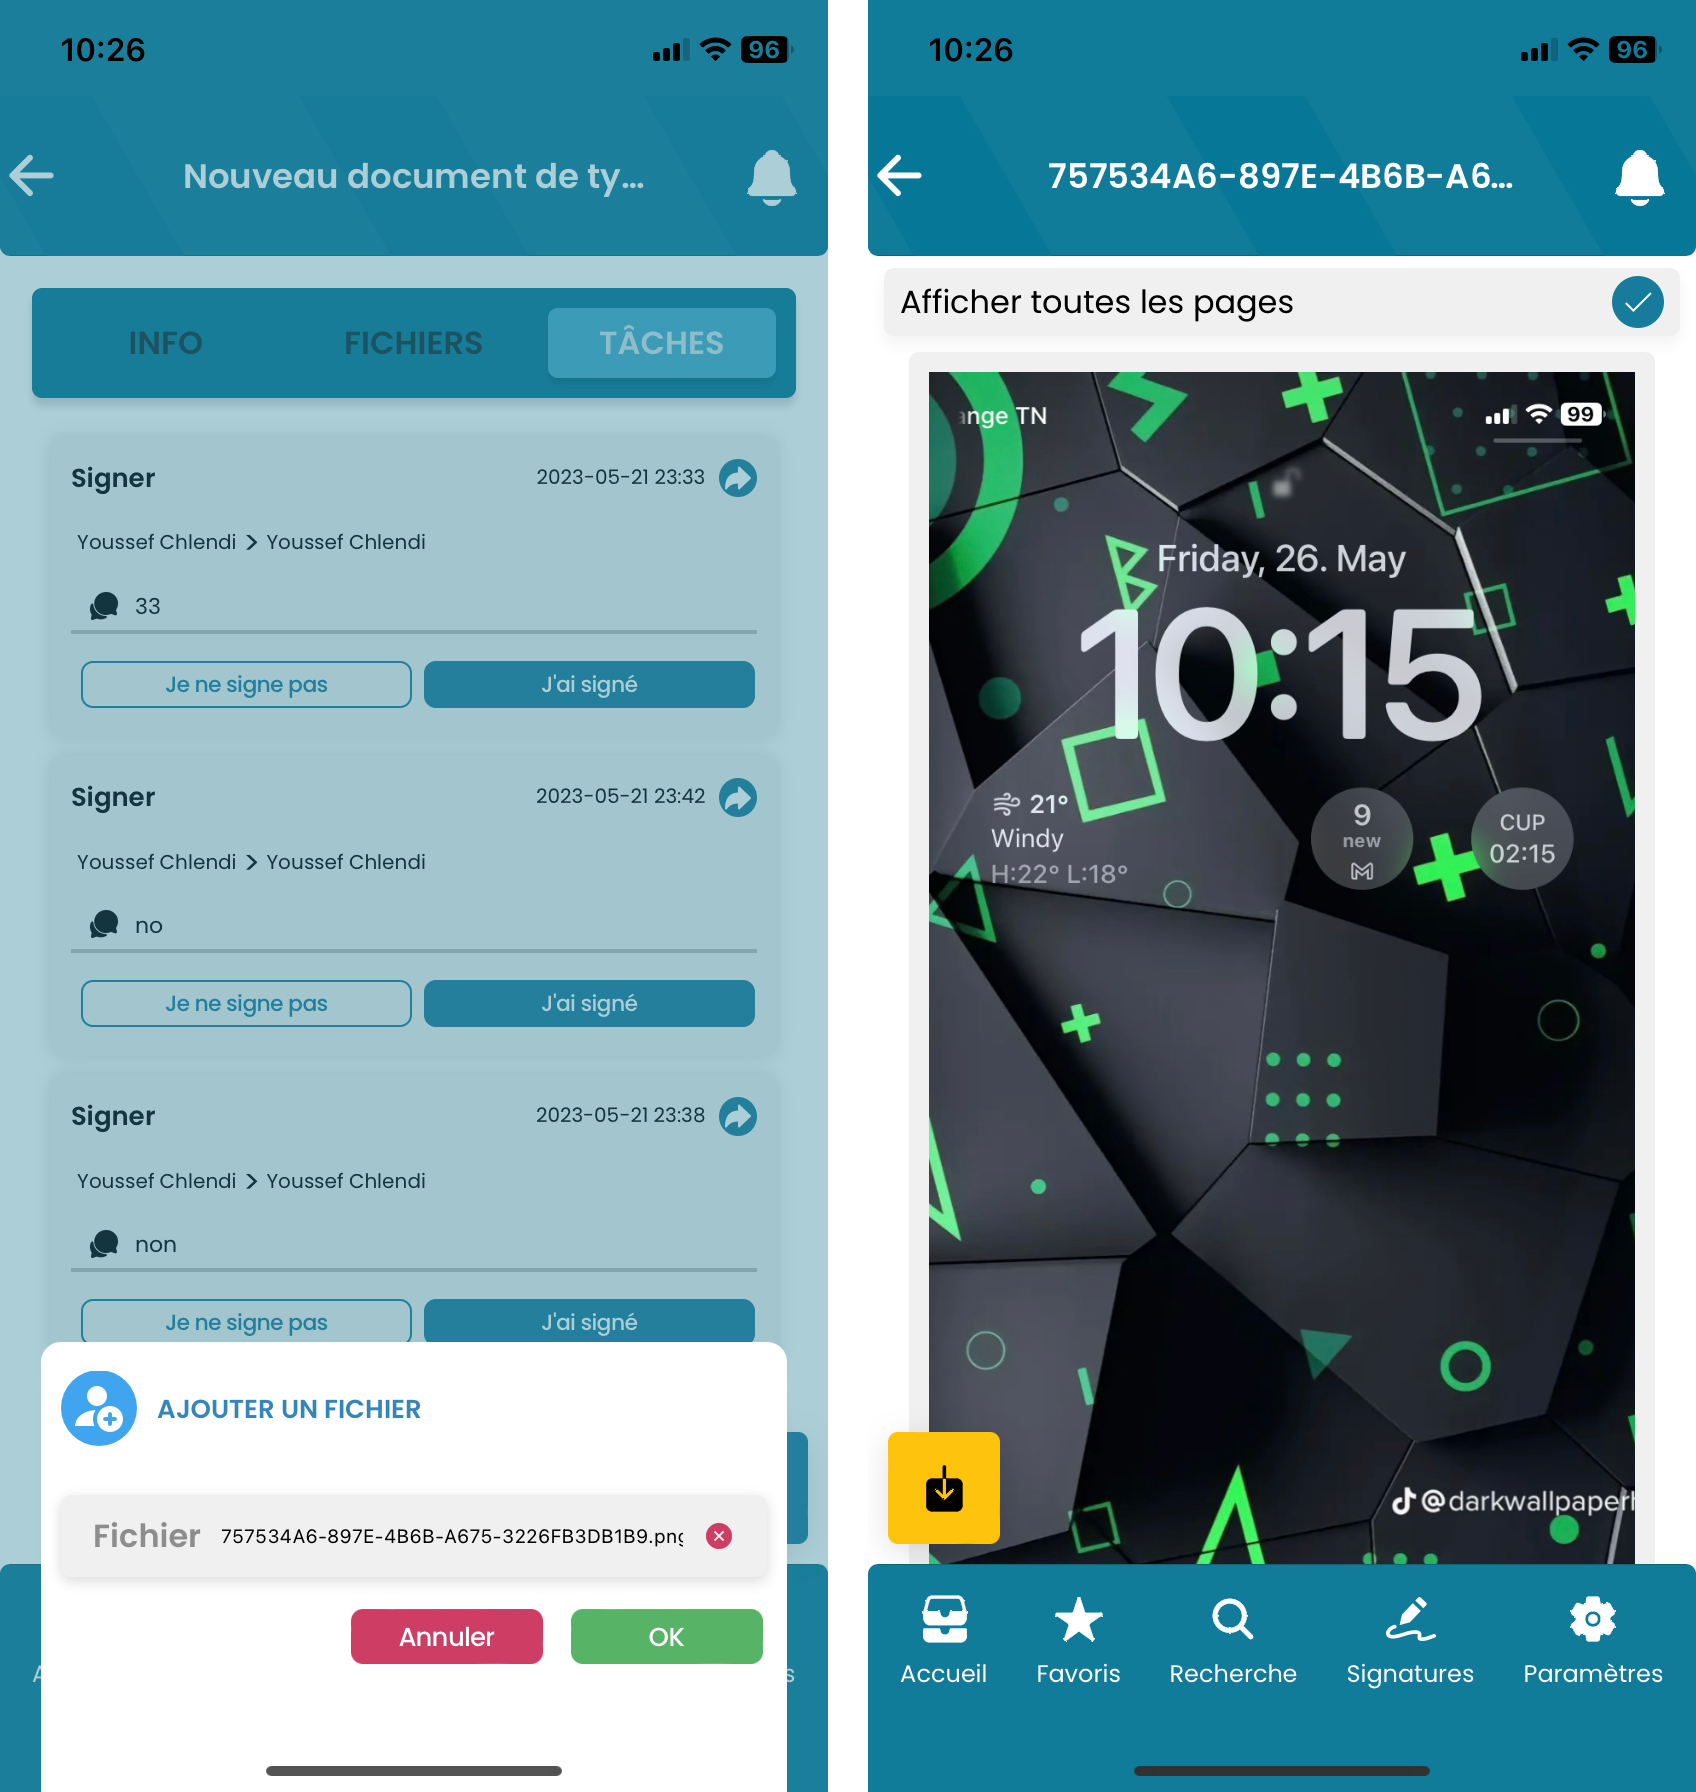
\includegraphics[width=0.4\textwidth]{upload_file_ios}}
    \caption{Quelques captures d'écran de l'ajout d'un fichier version IOS}
    \label{appendix:upload_file_ios}
\end{figure}

\begin{figure}[H]
    \centering
    \fbox{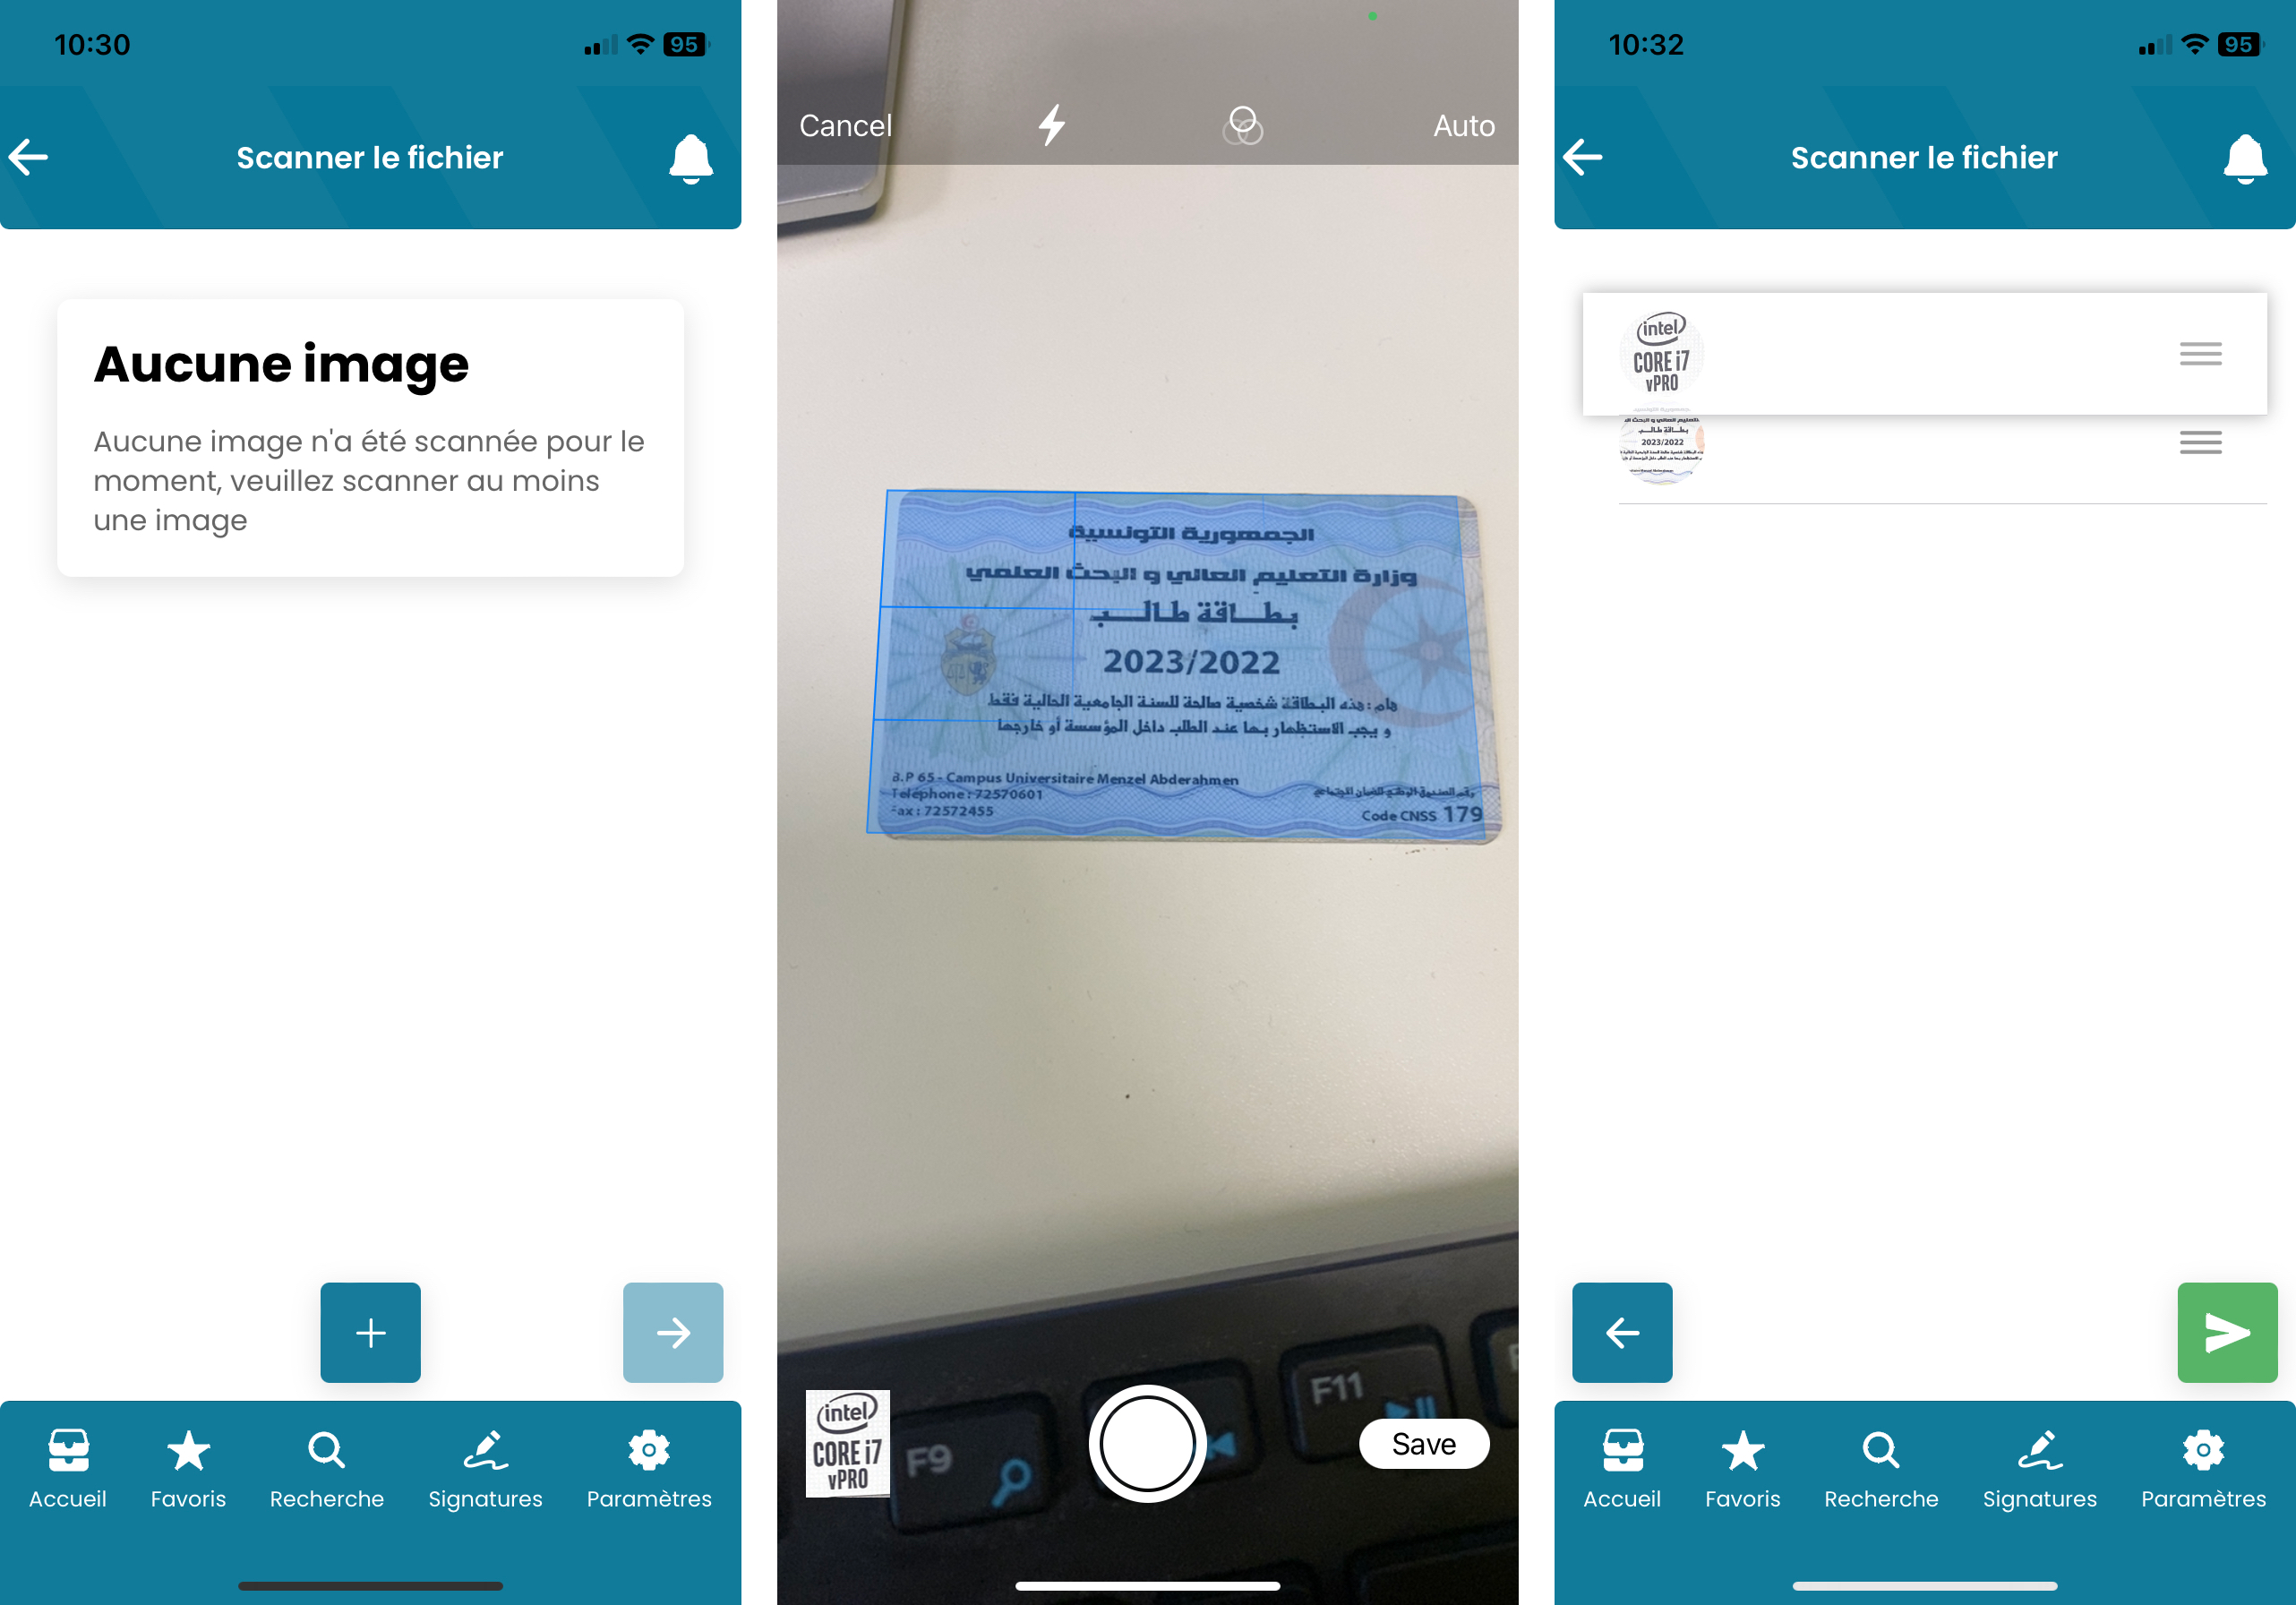
\includegraphics[width=0.4\textwidth]{add_file_scan_ios}}
    \caption{Quelques captures d'écran de l'ajout d'un fichier à l'aide de la caméra version IOS}
    \label{appendix:add_file_scan_ios}
\end{figure}

\subsection{Mode sombre}
\begin{figure}[H]
    \centering
    \fbox{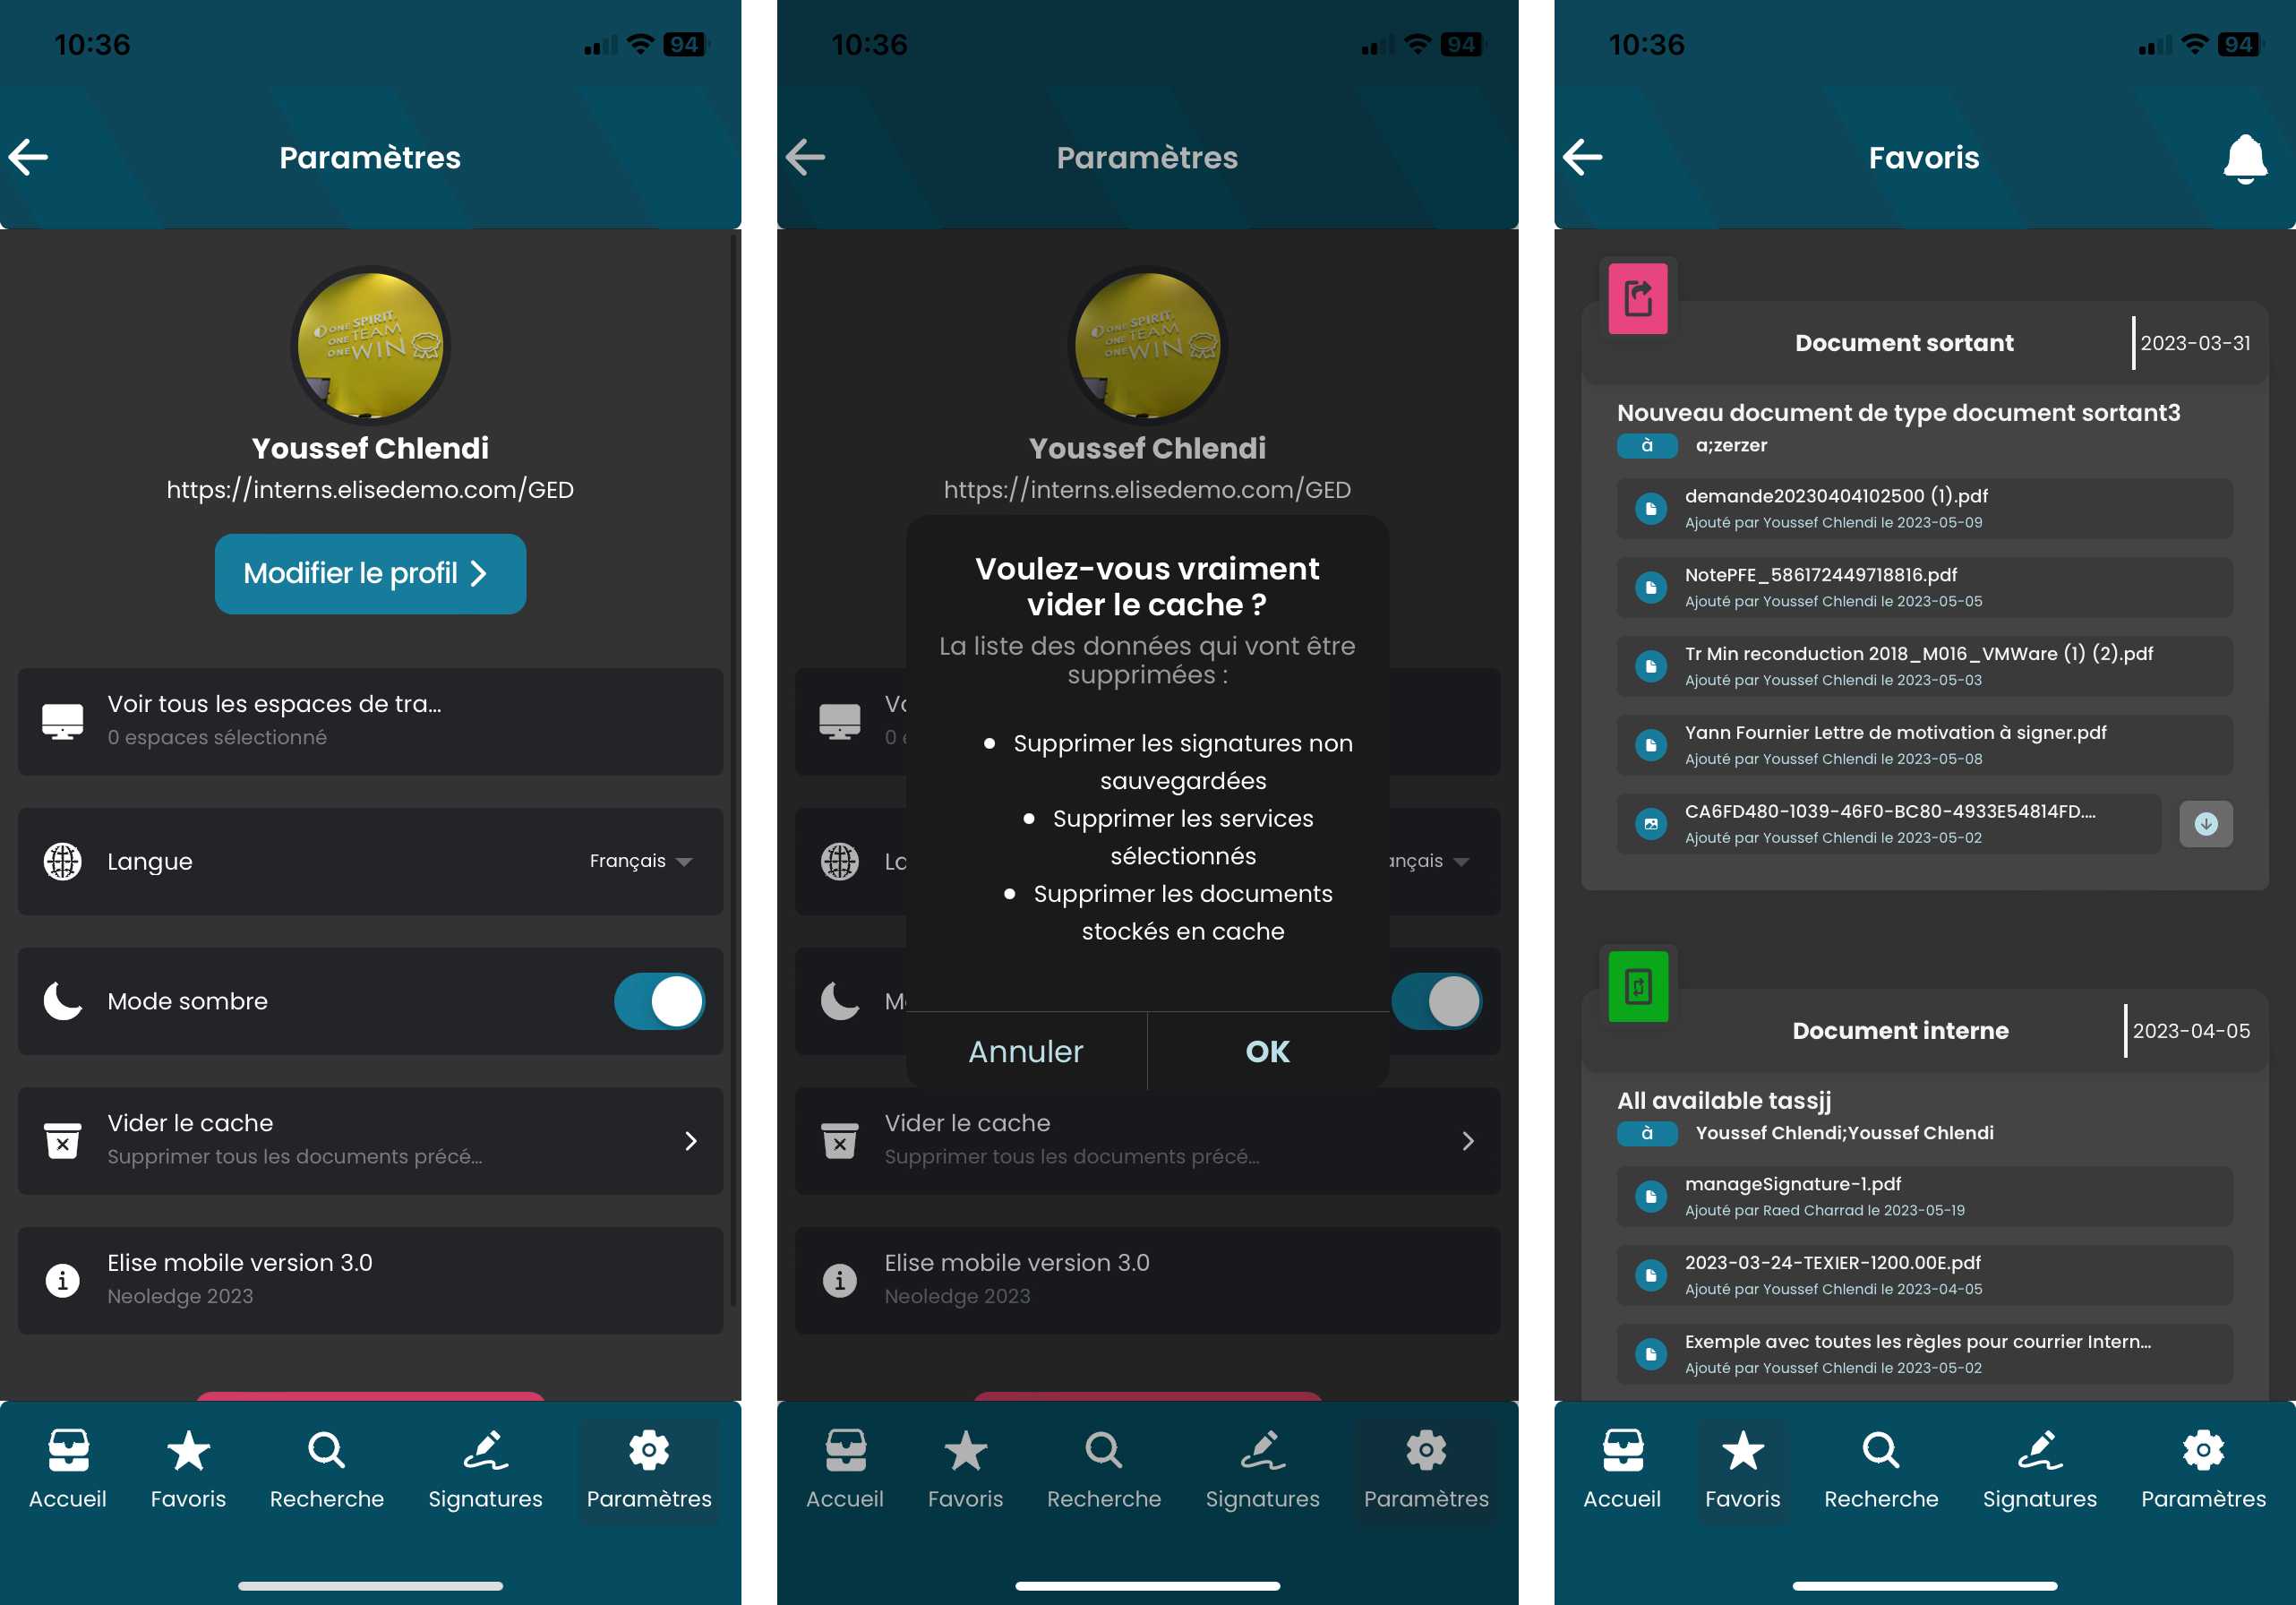
\includegraphics[width=0.4\textwidth]{sombre_ios}}
    \caption{Quelques captures d'écran de l'application version IOS en mode sombre}
    \label{appendix:capture_app1_ios}
\end{figure}
\label{appendix:sombre_ios}

\subsection{Verification biometrique}

\begin{figure}[H]
    \centering
    \fbox{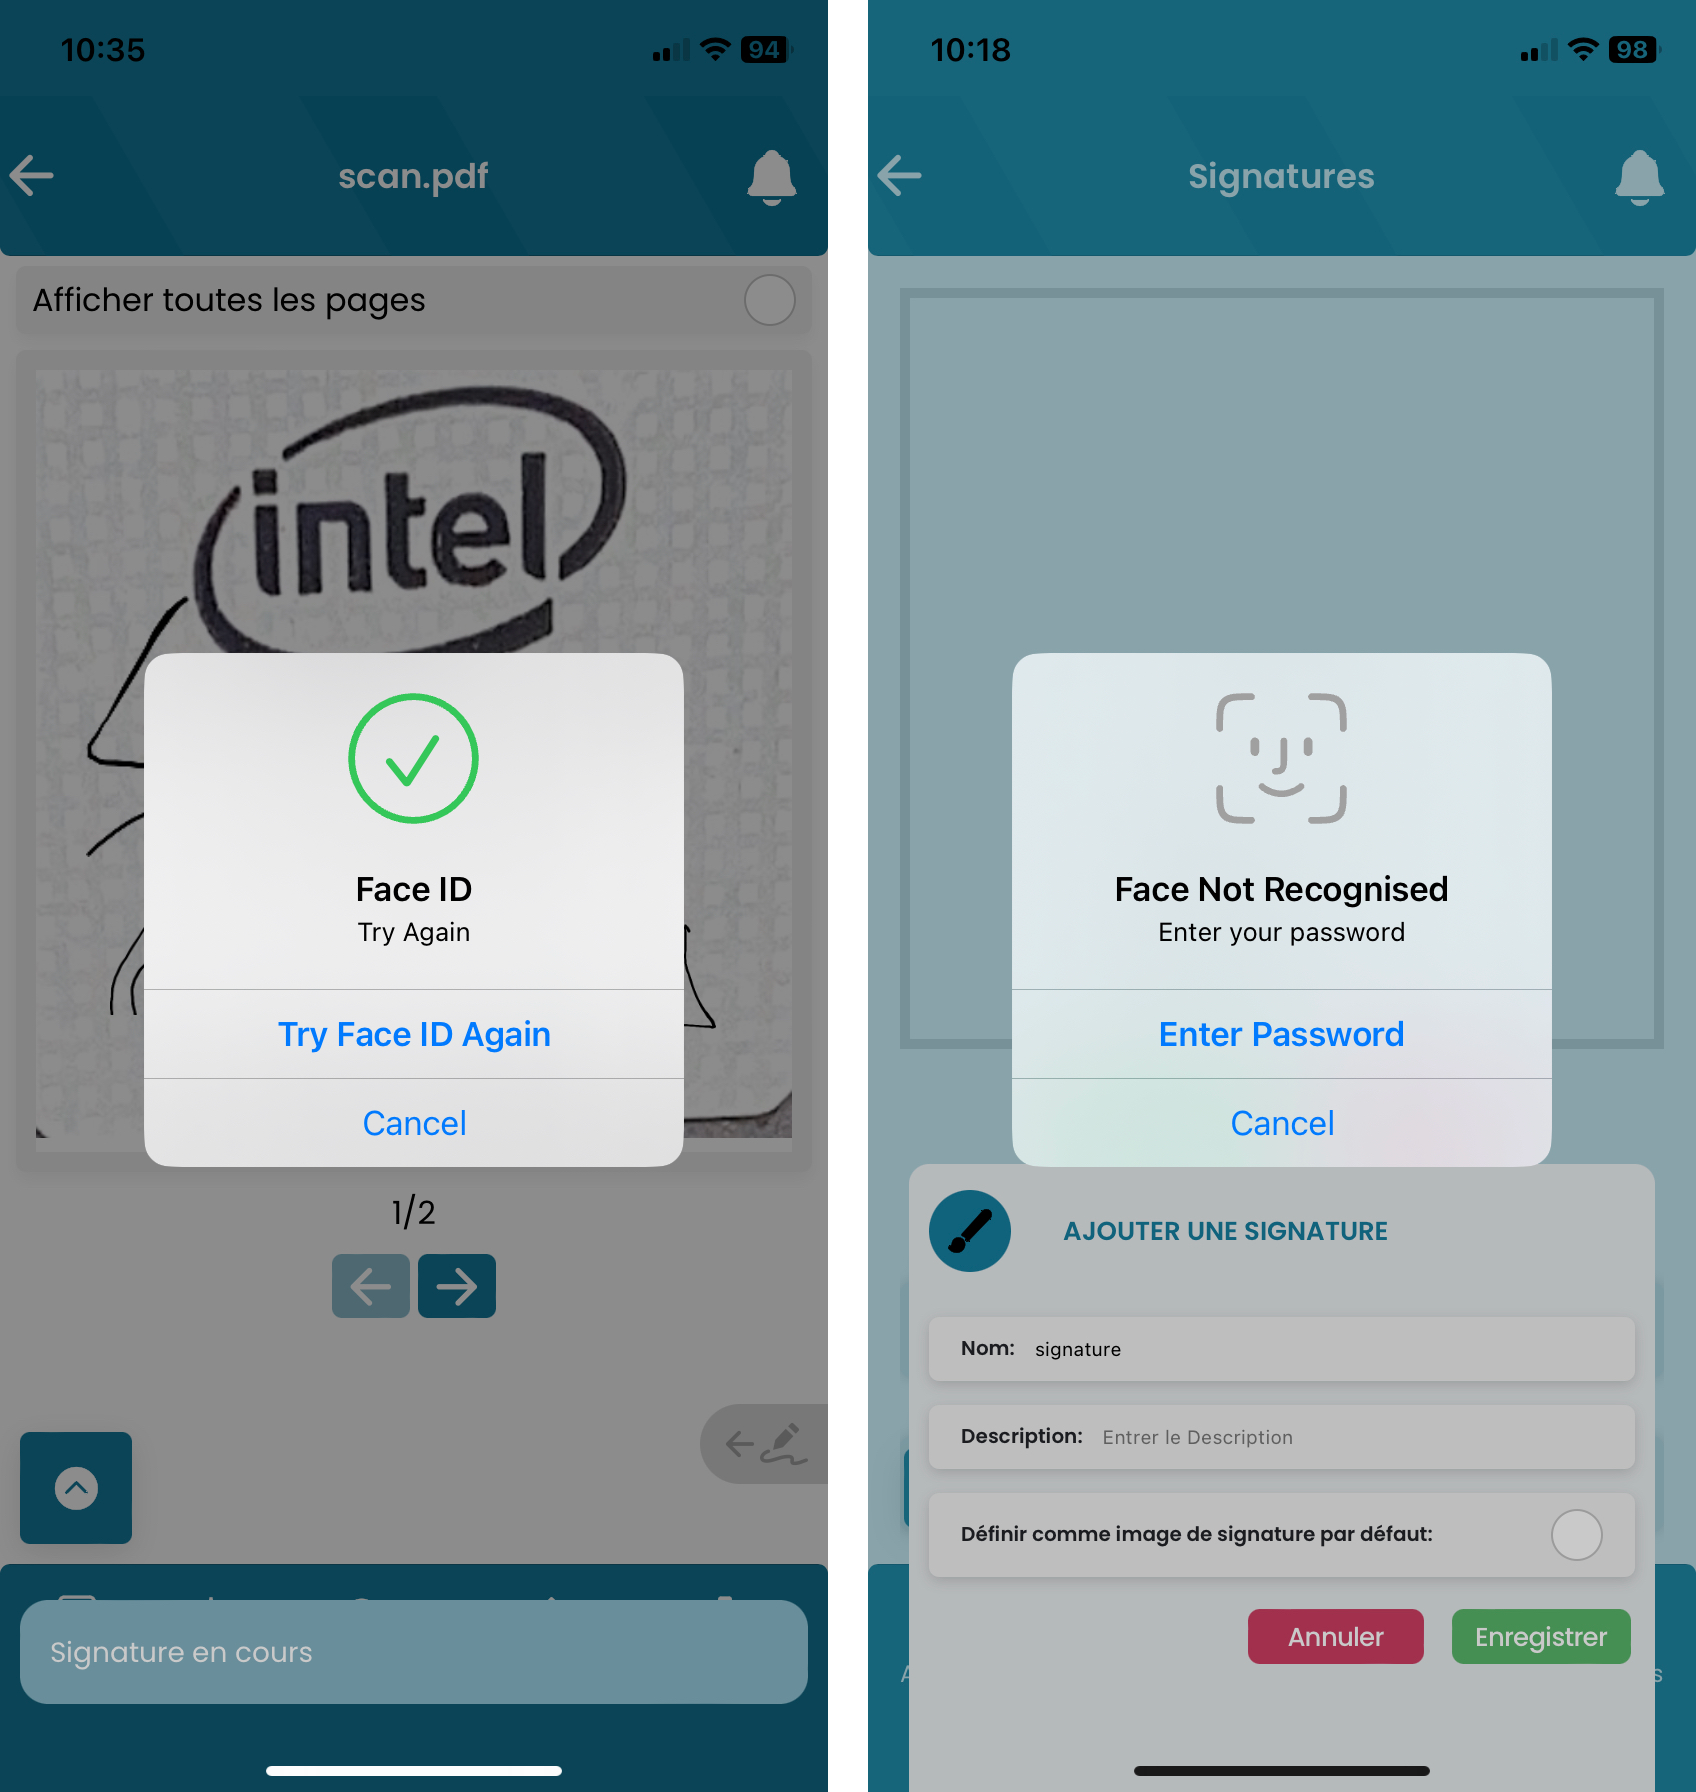
\includegraphics[width=0.4\textwidth]{biometrie_ios}}
    \caption{Quelques captures d'écran de la verification biometrique version IOS}
    \label{appendix:verification_biometrique}
\end{figure}





\section{Product backlog Azure DevOps}

\begin{figure}[H]
    \centering
    \fbox{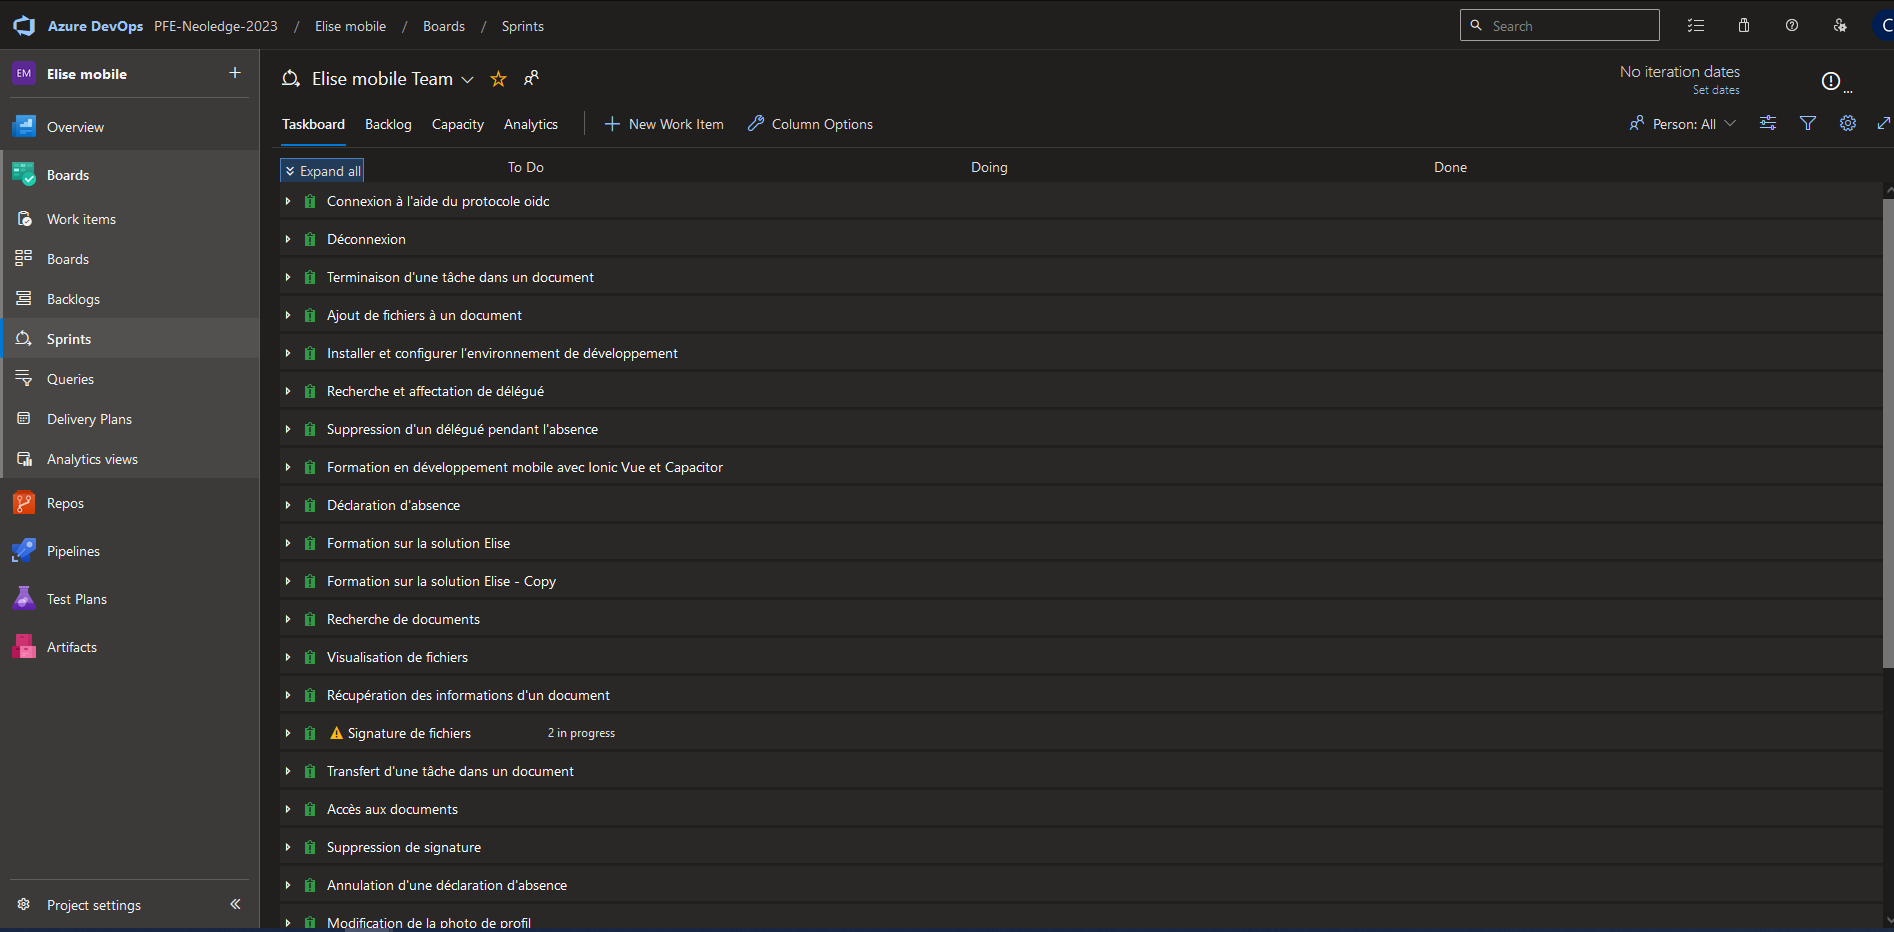
\includegraphics[width=0.8\textwidth]{capture_azure_devops}}
    \caption{Product backlog Azure DevOps}
    \label{appendix:product_backlog_azure_devops}
\end{figure}




\section{neo-pdf-viewer}
\label{appendix:neo-pdf-viewer}

\subsection{Fonctionnalité de l'affichage des images}

Pour prendre en charge les fichiers de type image dans notre package "neo-pdf-viewer", nous avons suivi les étapes suivantes :
\begin{itemize}
    \item \textbf{Ajouter un filtre de type de fichier :} Nous avons ajouté un filtre pour les fichiers de type image dans le composant "neo-pdf-viewer" pour mieux gérer les fichiers de différents types.
    \item \textbf{Ajouter un composant d'affichage d'image :} Nous avons utilisé le composant "img" de HTML pour afficher les images dans "neo-pdf-viewer".
\end{itemize}

L'ajout de la fonctionnalité d'affichage des images à "neo-pdf-viewer" nous a permis d'offrir une meilleure expérience utilisateur en affichant les images dans le même composant que les fichiers PDF.

\begin{figure}[H]
    \centering
    \fbox{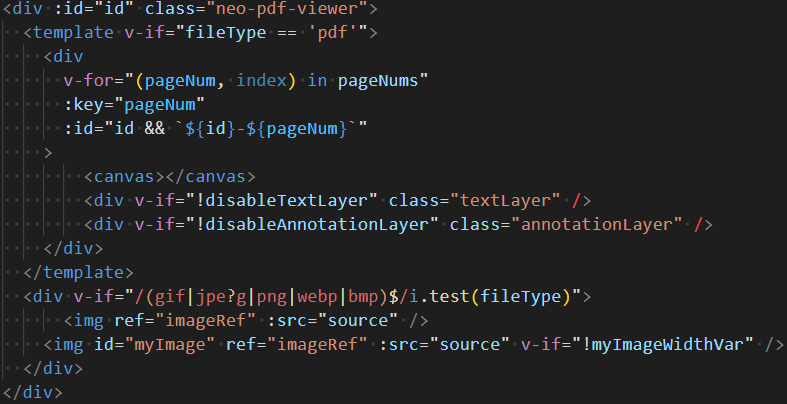
\includegraphics[width=0.8\textwidth]{code_image}}
    \caption{Code d'affichage des images}
    \label{appendix:codedisplayimage}
\end{figure}

\subsection{Fonctionnalité de zoom}

Pour intégrer cette fonctionnalité de zoom dans notre package "neo-pdf-viewer", nous avons suivi les étapes suivantes :
\begin{itemize}
    \item \textbf{Évaluation des besoins :} Nous avons identifié le besoin de permettre aux utilisateurs de zoomer sur les documents PDF affichés dans "neo-pdf-viewer". Après avoir étudié différentes options, nous avons choisi d'utiliser la bibliothèque "vue3-pinch-scroll-zoom" pour sa facilité d'intégration et ses fonctionnalités complètes.
    \item \textbf{Configuration du composant :} Nous avons intégré la bibliothèque "vue3-pinch-scroll-zoom" pour englober chaque page de fichier dans un composant de zoom. 
    \item Mise a jour du package "neo-pdf-viewer" 
\end{itemize}

L'ajout de la bibliothèque "vue3-pinch-scroll-zoom" à "neo-pdf-viewer" nous a permis d'offrir une fonctionnalité de zoom fluide et intuitive

\begin{figure}[H]
    \centering
    \fbox{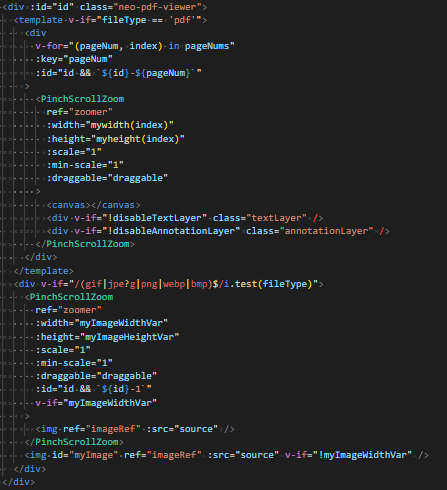
\includegraphics[width=0.7\textwidth]{capture_code_zoom}}
    \caption{Code de zoom}
    \label{appendix:zoom_code}
\end{figure}


% Démarrage de projet avec Firebase.
\section{Démarrage de projet avec Firebase}
\label{appendix:firebase_cloud_messaging}

La première étape pour démarrer un projet avec Firebase est de créer un projet sur la console Firebase. Pour ce faire, il suffit de se rendre sur le site web de Firebase et de cliquer sur le bouton "Ajouter un projet" comme illustré dans la figure \ref{appendix:firebase_create_project}.

\begin{figure}[H]
    \centering
    \fbox{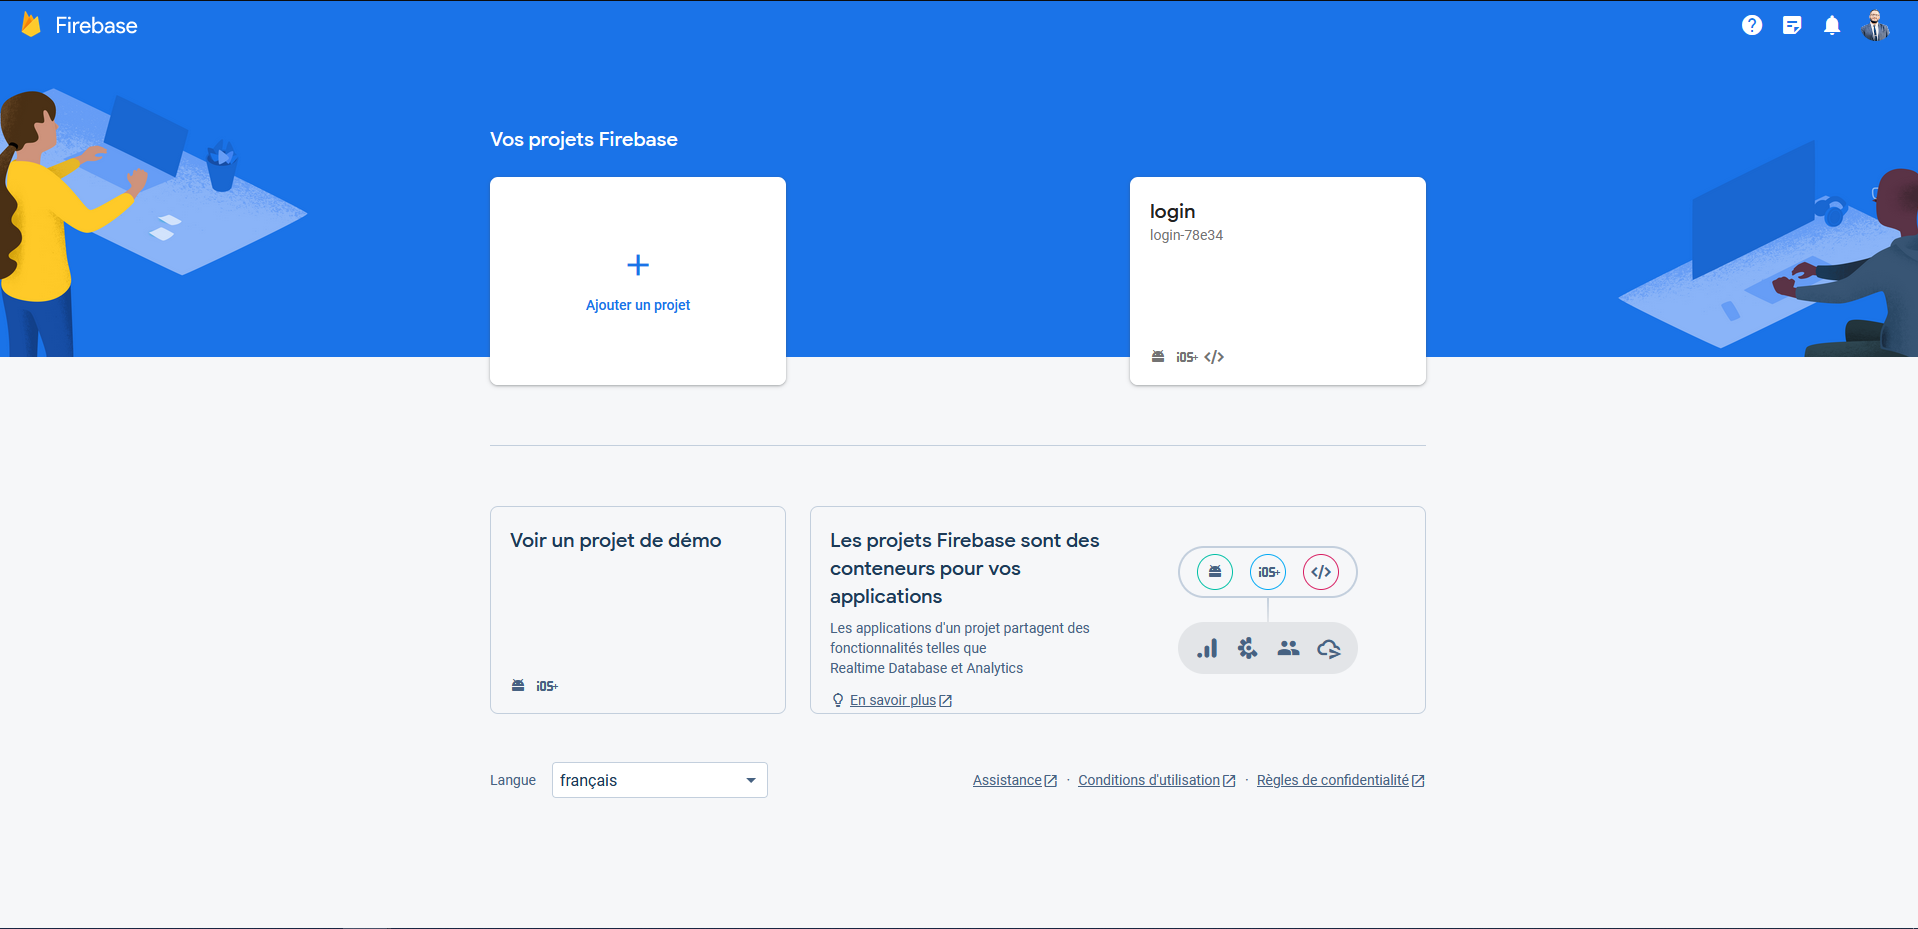
\includegraphics[width=0.8\textwidth]{firebase_create_project}}
    \caption{Création d'un projet sur Firebase}
    \label{appendix:firebase_create_project}
\end{figure}

Une fois le projet créé, il faut ajouter une application Android et une application IOS au projet. Pour ce faire, il faut cliquer sur le bouton "Ajouter une application" comme illustré dans la figure \ref{appendix:firebase_add_app}.

\begin{figure}[H]
    \centering
    \fbox{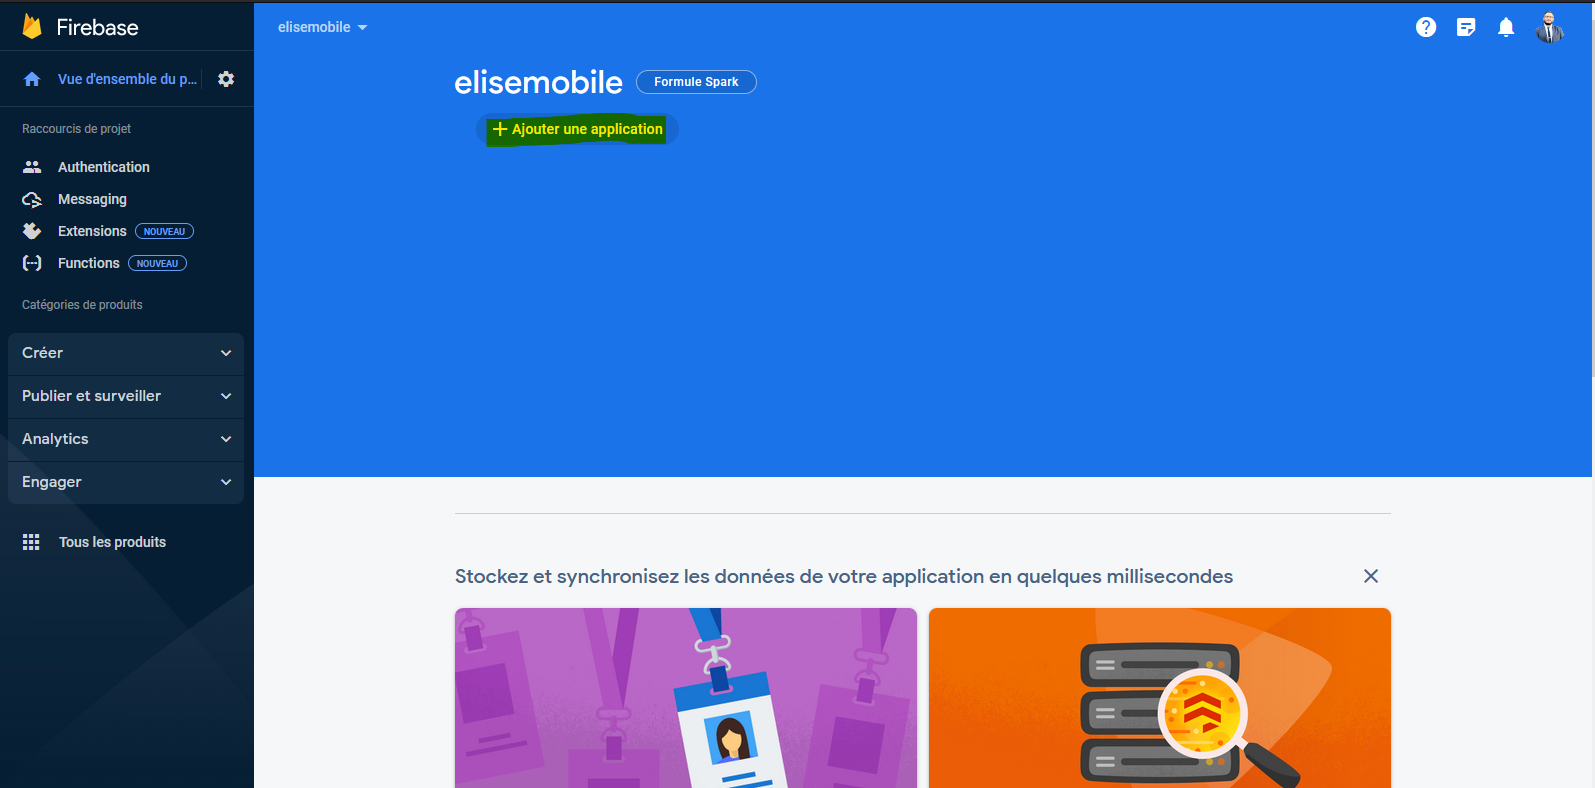
\includegraphics[width=0.8\textwidth]{firebase_add_app}}
    \caption{Ajout d'une application sur Firebase}
    \label{appendix:firebase_add_app}
\end{figure}

Une fois les applications ajoutées, il faut télécharger les fichiers de configuration pour chaque application et les ajouter au projet. Pour ce faire, il faut cliquer sur le bouton "Ajouter Firebase à votre application Android" ou "Ajouter Firebase à votre application IOS" comme démontré dans la démonstration dans la page d'ajout.

Pour suivre les étapes de configuration de Firebase Cloud Messaging dans une application Ionic Capacitor, il faut suivre les étapes décrites dans la documentation officielle de Capacitor \url{https://capacitorjs.com/docs/guides/push-notifications-firebase}.



% Backend notification
\section{Serveur backend de notification}
\label{appendix:backend_notification}

Le serveur backend de notification est une application Express.js qui utilise le package "FCM" pour envoyer des notifications aux utilisateurs.

\subsection{Les routes}

Le serveur backend de notification contient 3 routes :

\begin{table}[H]
    \caption{Les routes du serveur backend de notification}
    \label{appendix:backend_notification_routes}
    \centering
    \begin{tabular}{|l|l|p{6cm}|p{6cm}|}
    \hline
    Méthode & Route & Paramètres & Description \\ \hline
    POST & /send & token, uid, displayName, title, body, subtitle, click\_action, data & Envoie une notification à un utilisateur \\ \hline
    POST & /register & token, uid, displayName, language & Enregistre un utilisateur \\ \hline
    POST & /unregister & token, uid, displayName, language & Désenregistre un utilisateur \\ \hline
    \end{tabular}
    
\end{table}

\subsection{Structure du code}
La figure \ref{appendix:backend_notification_structure} illustre la structure du code du serveur backend de notification.

\begin{figure}[H]
    \centering
    \fbox{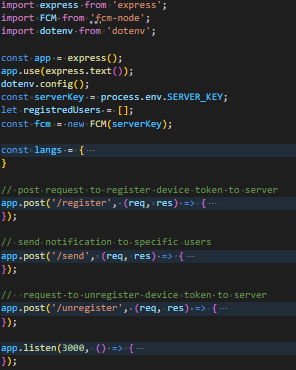
\includegraphics[width=0.8\textwidth]{backend_application}}
    \caption{Structure du code du serveur backend de notification}
    \label{appendix:backend_notification_structure}
\end{figure}


\subsection{Fonction d'envoi de notification}

La figure \ref{appendix:backend_notification_send} illustre la fonction d'envoi de notification du serveur backend de notification.

\begin{figure}[H]
    \centering
    \fbox{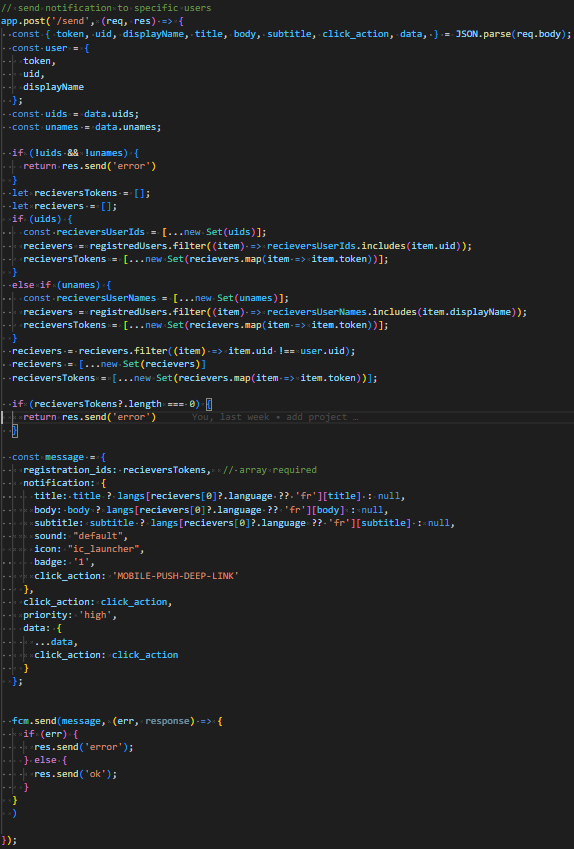
\includegraphics[width=0.8\textwidth]{send_notification_node}}
    \caption{Fonction d'envoi de notification du serveur backend de notification}
    \label{appendix:backend_notification_send}
\end{figure}
